% Adding a coloured vertical edge to the pages in the chapter
\ClearShipoutPicture
\AddToShipoutPicture{%
  \AtPageLowerLeft{%
    \checkoddpage
    \ifoddpage
      \begin{tikzpicture}[remember picture,overlay] % Odd page → right edge
        \draw[line width=80pt, colour_chapter5] 
             (\paperwidth,0) -- (\paperwidth,\paperheight);
      \end{tikzpicture}%
    \else
      \begin{tikzpicture}[remember picture,overlay] % Even page → left edge
        \draw[line width=80pt, colour_chapter5] 
             (0,0) -- (0,\paperheight);
      \end{tikzpicture}%
    \fi
  }%
}

%%%%%%%%%%%%%%%%%%%%%%%%%%%%%%%%%%%%%%%%%%%%%%%%%%%%%%%%%%%
\chapter{Flash-flood-focused verification of rainfall-based 
predictions of areas at risk of flash floods}
\label{flash_flood_focused_verification_rainfall_based_ff}
\graphicspath{{chapter_05/figures}{chapter_05/tables}}
%%%%%%%%%%%%%%%%%%%%%%%%%%%%%%%%%%%%%%%%%%%%%%%%%%%%%%%%%%%

\underline{\textbf{Authors' contribution for this chapter:}} Fatima M. Pillosu designed the study, with advice from Hannah Cloke and Christel Prudhomme, obtained the datasets, carried out the analysis, and led the writing of the manuscript. All authors assisted with writing the manuscript. Overall, 90\% of the writing was undertaken by Fatima M. Pillosu.

\vspace{\baselineskip}

\section*{PREFACE}
\addcontentsline{toc}{section}{PREFACE}

The first main analysis chapter (Chapter \ref{flash_flood_focused_verification_rainfall_based_ff}) undertakes the flash-flood-focused evaluation of short- and medium-range post-processed probabilistic point-scale rainfall forecasts. Such forecasts have been shown to predict better than the raw ERA5 flash-flood-triggering localised extreme rainfall events \citep{Pillosu_2025a}. While such an improvement in the prediction of localised extreme rainfall should enable the improved detection of areas at risk of flash floods, a flash-flood-focused assessment is fundamental to determining the extent to which enhanced rainfall prediction accuracy translates into meaningful improvements in flash flood hazard identification. In this chapter, \textcolor{colour_chapter5}{research question 1 (RQ1) "Can post-processed global NWP rainfall forecasts successfully identify areas at risk of flash floods up to medium-range lead times?"} is answered. Moreover, the first research component of this thesis is addressed, i.e. \textcolor{colour_chapter5}{developing a flash-flood-focused verification framework for predictions of areas at risk of flash floods, designed to benchmark the capability of different predictive systems}. Hence, this evaluation establishes a performance benchmark against which more sophisticated modelling approaches - incorporating additional hydrological and topographical parameters - can be measured. Such comparative analysis is essential for determining whether the increased computational demands and data requirements of complex systems yield commensurate improvements in flash flood prediction accuracy, or whether simpler precipitation-based approaches provide sufficient utility for early warning applications.

\clearpage

\section*{ABSTRACT}
\addcontentsline{toc}{section}{ABSTRACT}

\clearpage



%%%%%%%%%%%%%%%%%%%%%%
\section{Introduction}

Flash floods cause significant societal, economic, and environmental impacts \citep{Dordevic_2020}. These events arise through two primary mechanisms. The first involves intense, short-duration rainfall events (typically less than 6 hours) that generate rapid surface runoff and channel response, particularly over steep slopes. The second occurs when sustained moderate-to-extreme rainfall over extended periods (> 6 hours) progressively saturates soils, reducing infiltration rates and promoting surface runoff that inundates low-lying areas \citep{Speight_2021}. Short-duration flash flood events typically result from small-scale convective systems, whilst prolonged events are more frequently associated with large-scale, mesoscale convective systems or hurricanes \citep{Doswell_2001}. The distinction between these mechanisms is essential as they exhibit different temporal scales, spatial patterns, and relationships with antecedent catchment conditions, and predictability limits. This study aims to enhance preparedness and mitigation strategies against this escalating threat, particularly in regions with limited resources and data, by assessing the effectiveness of global rainfall forecasts in identifying areas at risk of flash floods.

\begin{tcolorbox}[
  colframe=colour_chapter5, % Use the custom HEX colour for the vertical line
  colback=white,            % Background colour remains white
  sharp corners,            % Ensures sharp edges
  boxrule=2mm,              % Thickness of the left vertical line
  left=0mm,                 % Space inside the left margin
  right=0mm,                % No space on the right
  toprule=0mm,              % Remove the top border
  bottomrule=0mm,           % Remove the bottom border
  rightrule=2mm            % Remove the right border
]
{\color{colour_chapter5} {\setlength{\parindent}{1.0em} The term \textbf{"identification of areas at risk of flash floods"} refers to the \textit{prediction of polygons - or areas - that might experience flash flooding due to the expected rainfall}.}}
\end{tcolorbox}

Forecast-triggered mitigation strategies, such as early warning systems \citep{CoughlanDePerez_2022, ŠakićTrogrlić_2022} and forecast-based financing protocols \citep{Bischiniotis_2019a, Perez_2016}, have been shown to improve resilience, decrease mortality, and lower recovery costs against riverine floods. Yet, these strategies hinge on accurate, timely predictions. In lower-income countries, accurate forecasts with even longer lead times are required to set cost-effective mitigation strategies \citep{Bazo_2019, Kiptum_2023}. 

Over the years, flash flood forecasting systems have been developed at local/regional \citep{Speight_2018, Corral_2019, Ibarreche_2020, RamosFilho_2021, Shuvo_2021}, national \citep{Javelle_2016, Liu_2018}, and continental scales \citep{Gourley_2017, Raynaud_2015}, with varying degrees of model complexity and forecast accuracy. These systems share a reliance on high-density rainfall and discharge observations, and km-scale rainfall forecasts \citep{Braud_2014}. This approach has prevented the development of a flash flood forecasting system that provides medium-range forecasts over a continuous global domain. Radar-derived rainfall predictions remain limited to a few hours ahead \citep{Imhoff_2022}, and kilometre-scale forecasts show substantial skill reduction beyond two days \citep{Barrett_2019}. Moreover, the uneven spatial distribution of these data sources restricts flash flood prediction to a collection of separate regional and national systems, including WMO's "Flash Flood Guidance System with Global Coverage" \citep{Georgakakos_2022}. Consequently, many areas of the world remain without access to flash flood guidance, highlighting the need for alternative approaches to address the challenge of providing medium-range predictions of areas at risk of flash floods over a continuous global domain.

Global NWP models, such as ECMWF’s IFS, are increasingly seen as a viable solution to this challenge. These models provide daily global rainfall predictions up to medium-range leads but have historically struggled to accurately predict extreme localised rainfall events due to their coarse resolution and parametrisation schemes \citep{Emerton_2016, Wen_2021}. Owing to recent improvements in global NWP forecast accuracy \citep{Haiden_2023, Lavers_2021}, the interest in using them to provide flash flood guidance in data-scarce regions and extend predictions’ lead times has recently increased \citep{Bucherie_2022b}. Additionally, the development of state-of-the-art post-processing techniques can enhance the quality of raw forecasts and make them more suitable for flash flood prediction \citep{Vannitsem_2021}. For example, the ecPoint statistical post-processing technique transforms global grid-based forecasts into probabilistic point-scale predictions, improving the reliability and discrimination ability of rainfall forecasts up to day 10, especially for extremes \citep{Hewson_2021}.

Since a significant gap remains in leveraging global rainfall NWP forecasts for flash flood forecasting, this study aims to bridge this gap by evaluating the performance of ERA5-ecPoint rainfall forecasts in identifying areas at risk of flash floods. The CONUS, with its extensive collection of flash flood impact reports within NOAA's Storm Event Database and its varying climate, serves as an ideal test bed for this research. The research question posed in this study is \textit{can post-processed global NWP rainfall forecasts successfully identify areas at risk of flash floods up to medium-range lead times?} The innovation proposed by this research is twofold. It first proposes a flash-flood-focused verification framework for predictions of areas at risk of flash floods, in recognition of the non-linear relationship between flash floods and triggering rainfall events. Hence, this framework can be used as a common framework to benchmark the general capabilities of different systems to predict areas at risk of flash floods. This research also provides a performance benchmark against which more sophisticated modelling approaches - incorporating additional hydrological and topographical parameters - can be measured. Such comparative analysis is essential for determining whether the increased computational demands and data requirements of complex systems yield commensurate improvements in flash flood prediction accuracy, or whether simpler precipitation-based approaches provide sufficient utility for early warning applications.

This chapter is organised as follows. Sections \ref{flash_flood_focused_verification_rainfall_based_ff_DATA} and \ref{flash_flood_focused_verification_rainfall_based_ff_METHODS} describe the data and methods used to develop the flash-flood-focused verification framework. Section \ref{flash_flood_focused_verification_rainfall_based_ff_RESULTS} presents the results of the objective verification analysis, while section \ref{flash_flood_focused_verification_rainfall_based_ff_CASE_STUDY} presents results from a case-study-based subjective verification analysis. Section \ref{flash_flood_focused_verification_rainfall_based_ff_DISCUSSIONS} discusses the verification results, while section \ref{flash_flood_focused_verification_rainfall_based_ff_CONCLUSIONS} draws concluding remarks for the study.


%%%%%%%%%%%%%%
\section{Data}
\label{flash_flood_focused_verification_rainfall_based_ff_DATA}


\subsection{Study domain}

This research establishes the CONUS as the primary study domain (see Figure \ref{fig:conus_domain}). The CONUS domain presents diverse hydro-meteorological conditions, encompassing varied topographical features ranging from coastal plains to mountainous terrain, and climatic regimes spanning Mediterranean, continental, subtropical, and desert classifications. This diversity encompasses a broad spectrum of flash-flood-generating mechanisms, ranging from intense convective precipitation to rain-on-snow events, thereby enhancing the potential for future transferability to global applications.

\begin{figure}[htbp]
\centering
\includegraphics[scale=0.65]{conus_domain_orography.png}
\caption{\textbf{CONUS domain.} The figure shows the orography at 1 km resolution (in shades of green and brown) and the location of the 25 most populated cities (black dots) over the CONUS.}
\label{fig:conus_domain}
\end{figure}

\subsection{Observations: NOAA's Storm Event Database}

The selection of the CONUS as the primary domain also lies on the high quality and comprehensiveness of NOAA's Storm Event Database. This database systematically records flash flood occurrences with high spatial and temporal resolution, including crucial metadata regarding impact severity, affected areas, and casualty information. The database's consistent reporting protocols and rigorous quality control procedures mitigate the observational uncertainty that typically plagues flash flood research \citep{Panwar_2020}.

The Storm Event Database serves as the US's official repository of severe weather records, including flash floods. Flash flood records began in 1996, with significant improvements in geographical precision implemented in 2007, when reporting transitioned from county-level to polygon-based representation, later extended to reports from 2001\footnote{\url{https://inside.nssl.noaa.gov/flash/database/}}.

The database covers the entire United States and territories with a spatial bounding box from 172.0°W to 65.0°E longitude and 18.0°N to 72.0°N latitude\footnote{\url{https://www.ncei.noaa.gov/access/metadata/landing-page/bin/iso?id=gov.noaa.ncdc:C00510}}. Data collection involves a network of 123 Natioanl Weather Service Forecast Offices gathering information from emergency management officials, law enforcement, trained SKYWARN spotters, damage surveys, media reports, and public observations\footnote{\url{https://www.ncdc.noaa.gov/stormevents/faq.jsp}}.

The Storm Event provides extensive metadata for flash flood events. Among all the available keys, we considered in this study only the keys described in table 3. Although professional meteorologists and hydrologists collect flash flood reports to include in the Severe Storm Database, any human augmented reporting system is subject to variations in population density, diurnal cycles of human activity, and more mundane transcription or memory errors that affect the timing and location of reports \citep{Barthold_2015}. Evidence of these issues has been found in assessments of FFG skill \citep{Clark_2014}, and it has been found that the distribution of SED's flash floods reports is affected by the distribution of human population \cite{Marjerison_2016}. 

\begin{figure}[htbp]
\centering
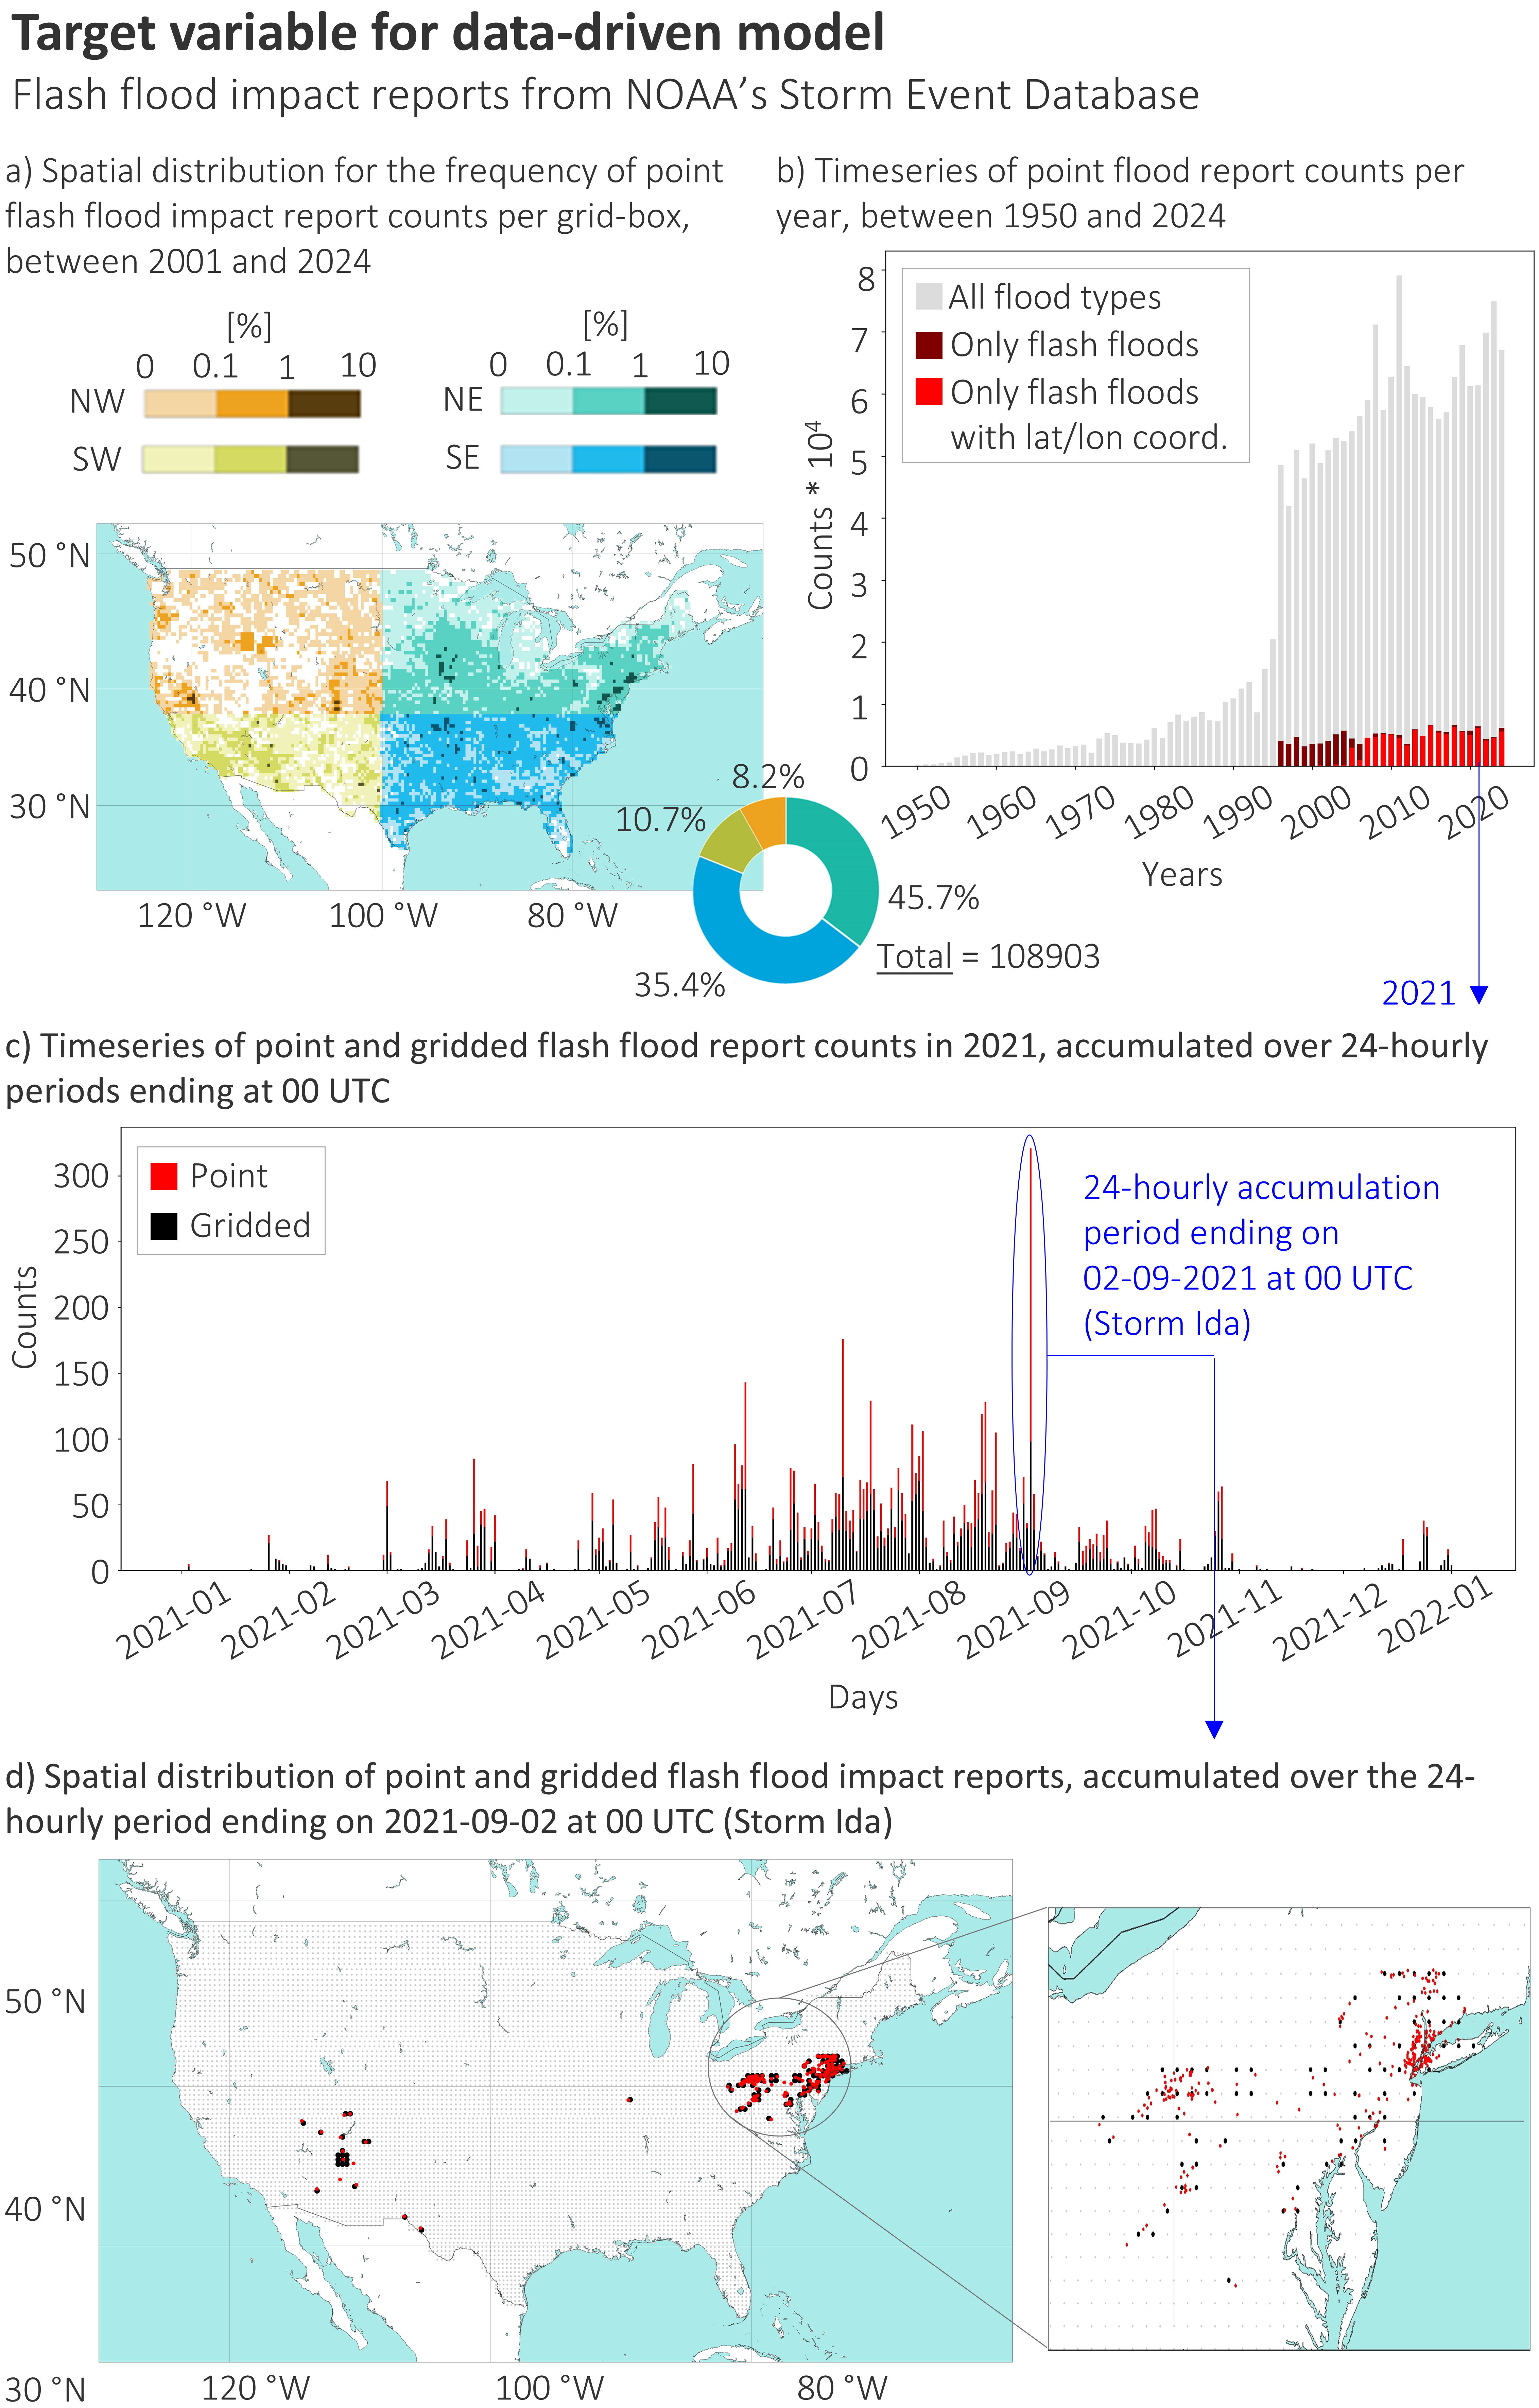
\includegraphics[width=\textwidth]{sed_ff_reports.png}
\caption{\textbf{Flash flood reports from NOAA's Storm Event Database.} Panel (a) displays the timeseries of flood reports from 1950 to 2024, distinguishing between all flood types (grey bars), only flash floods (dark red bars), and only flash flood reports with latitude/longitude coordinates (bright red bars) for the period 2001-2024. Panel (b) presents the spatial distribution of point flash flood report frequency per grid box for the period 2001-2024, shown as percentages (\%) across four geographical quadrants (North-West (NW, in shades of orange), South-West (SW, in shades of yellow), North-East (NE, in shades of green), South-East (SE, in shades of blue)) of the CONUS. The pie chart indicates the relative proportion of reports by region, with a total of 108,903 flash flood events reported in the considered period. Panel (c) illustrates the daily distribution of flash flood reports throughout 2021, showing both point reports (red bars) and gridded reports (black bars) accumulated over 24-hour periods ending at 00 UTC. The highlighted date with the blue circle (2nd September 2021) corresponds to the flash flood reports recorded during Storm Ida. Panel (d) maps the spatial distribution of flash flood reports, accumulated over the 24-hourly period ending at 00 UTC on 2 September 2021, displaying point reports with red dots and gridded reports with black dots. The zoomed-in box shows the reports recorded on the NE coast during Storm Ida.}
\label{fig:conus_domain}
\end{figure}

In this study, we are using version 3.1 of the database, and we consider only reports over the CONUS that go from 2001 to 2024. 


%%%%%%%%%%%%%%%%%
\section{Methods}
\label{flash_flood_focused_verification_rainfall_based_ff_METHODS}


%%%%%%%%%%%%%%%%%
\section{Results}
\label{flash_flood_focused_verification_rainfall_based_ff_RESULTS}

%%%%%%%%%
\subsection{Assessment of rainfall-based predictions of areas at risk of flash floods}
\label{verif_rainfall_based_fc}

\subsubsection{Overall verification scores: frequency bias and area under the ROC curve}

\begin{figure}[htbp]
\centering
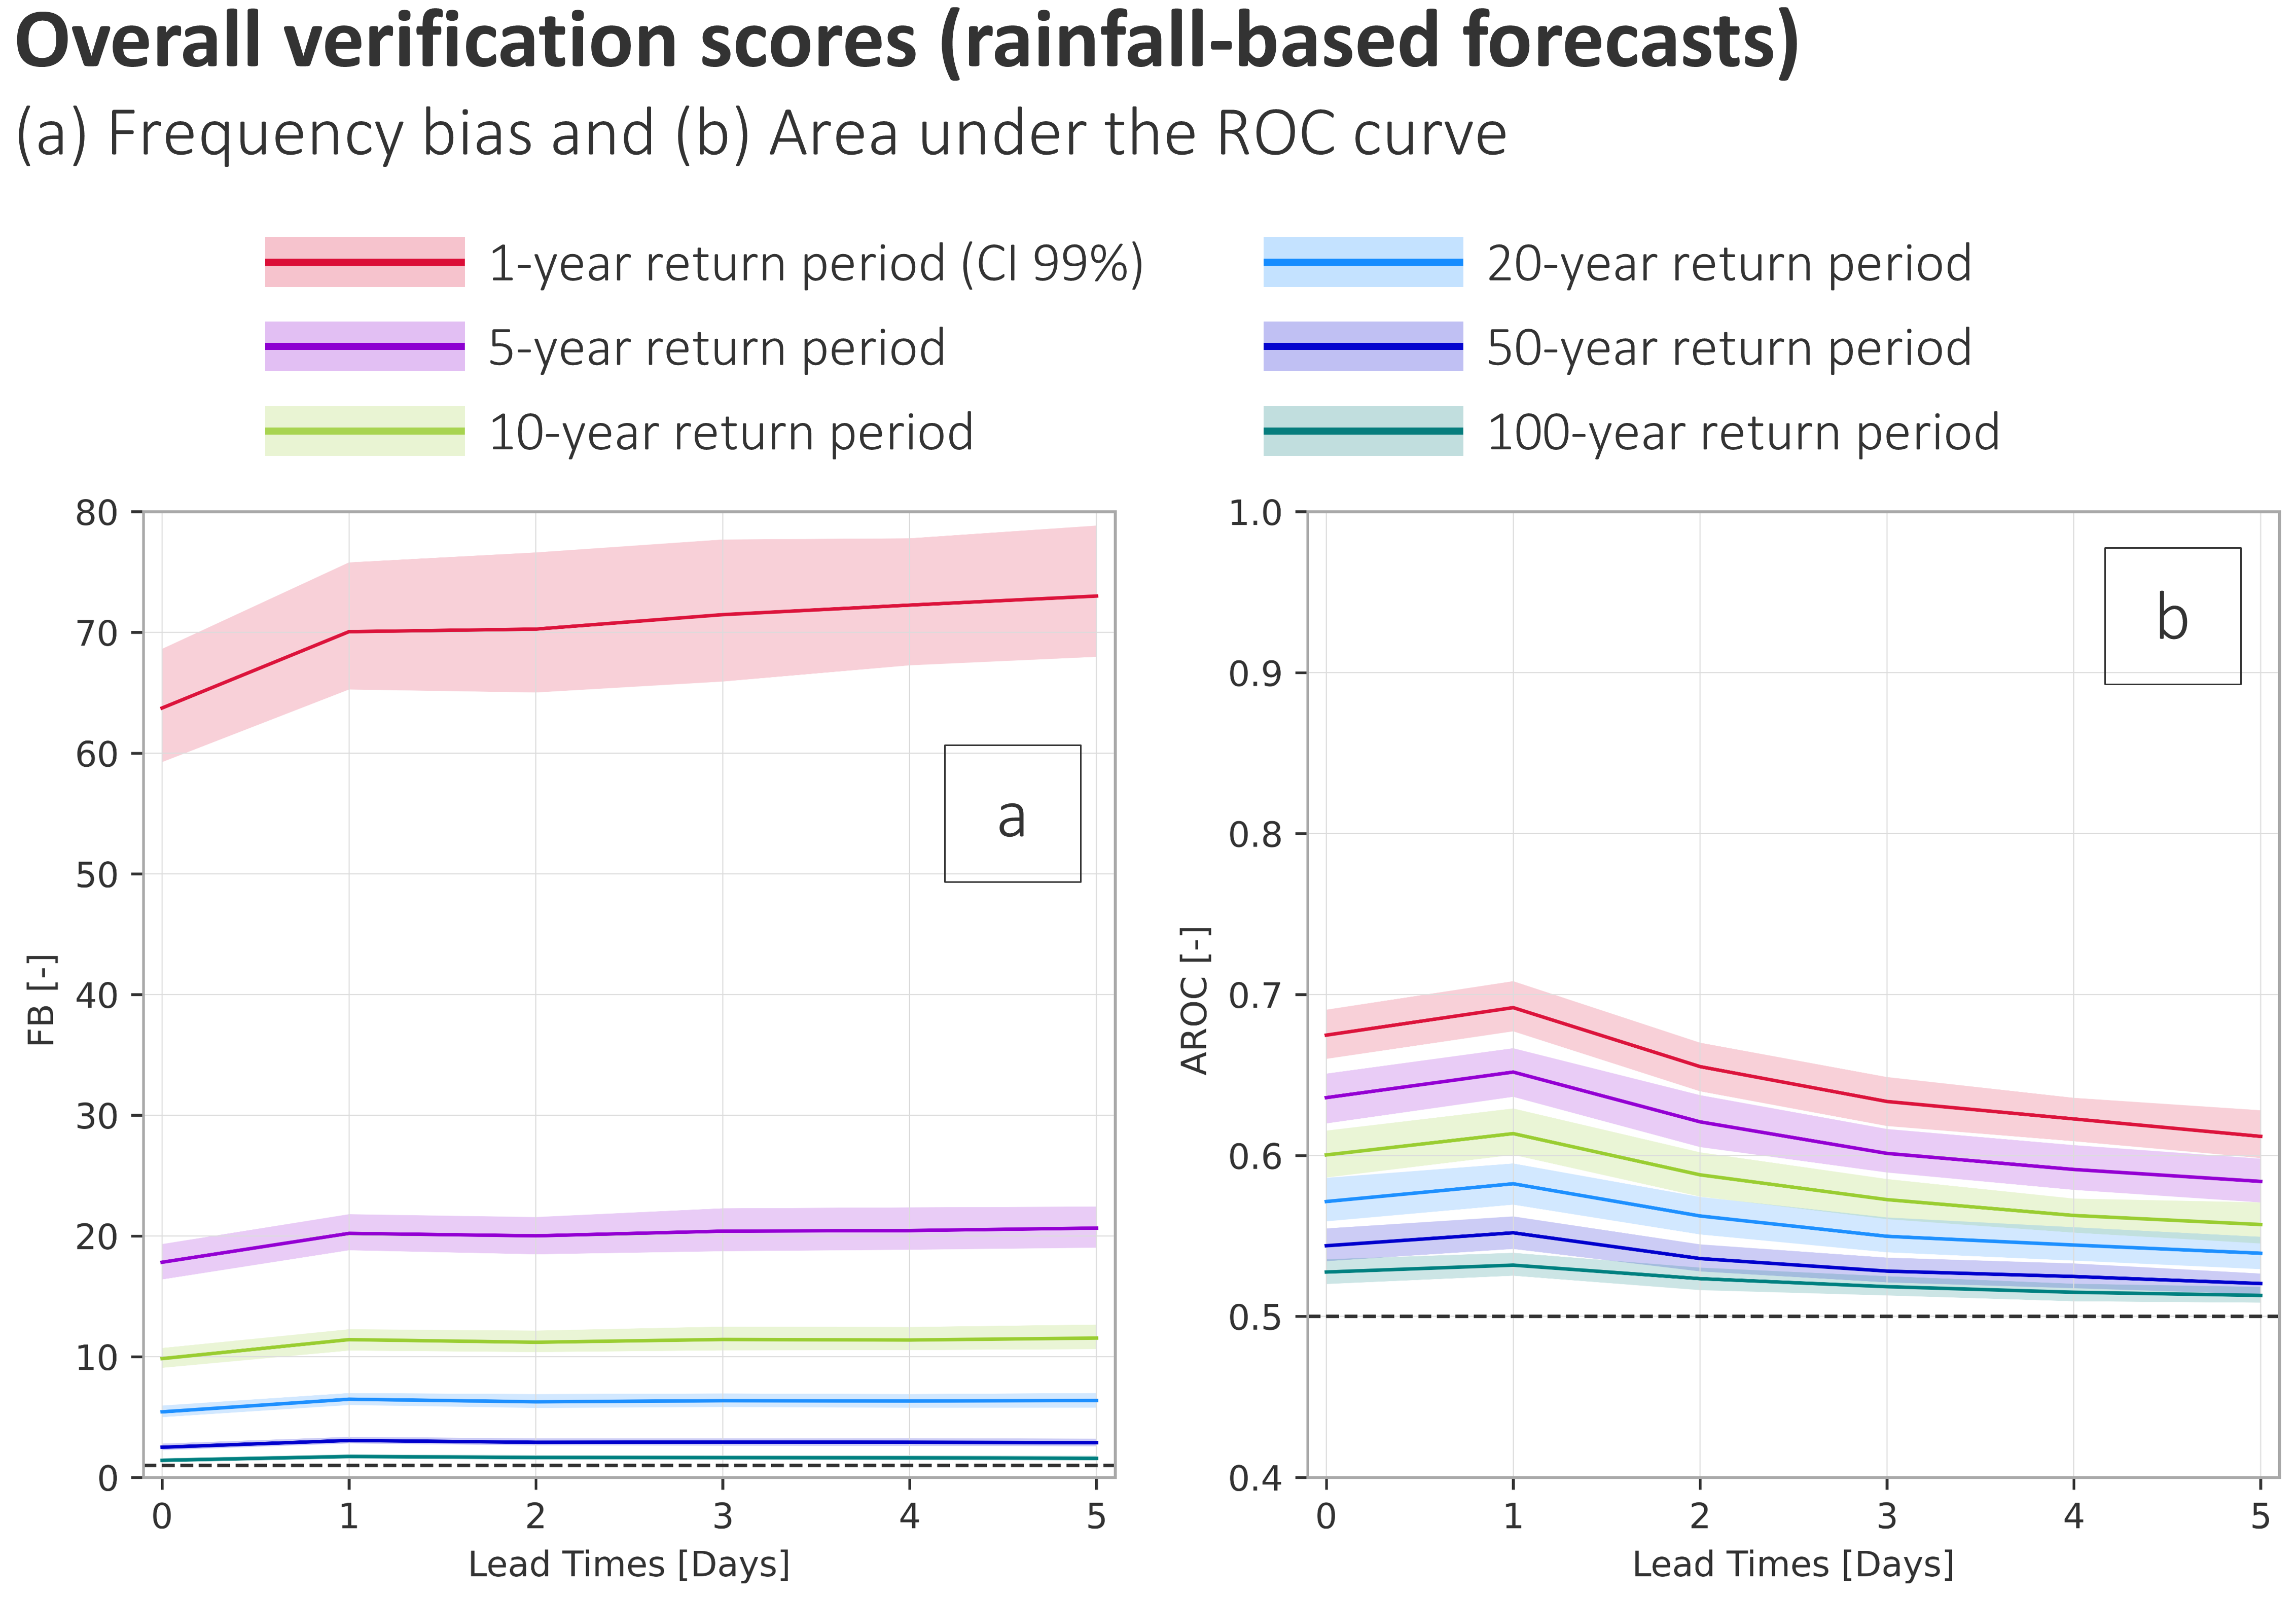
\includegraphics[width=\textwidth]{chapter_05/figures/rainfall_based_ff_verif_overall_scores.png}
\caption{\textbf{Overall verification scores for the rainfall-based forecasts of areas at risk of flash flood.} Panel (a) shows the frequency bias (solid lines) for 1-year (in red), 5-year (in purple), 10-year (in light green), 20-year (in cyan), 50-year (in blue), and 100-year return period (in green). The corresponding shaded areas represent the confidence intervals at 99\% confidence level. The inset box contains a zoomed-in version of the panel to show better the frequency bias values close to 1 (representing perfect bias). Panel (b) shows the area under the ROC curve.}
\label{fig:rainfall_based_ff_verif_overall_scores}
\end{figure}


\subsubsection{Discrimination ability}

All forecasts for rainfall events exceeding the 1-year return period threshold (Figure \ref{fig:rainfall_based_ff_verif_breakdown_scores_roc_1rp}) exhibit a discrimination ability superior to random chance, as the curves are above the diagonal reference line. A systematic degradation in discrimination ability is observed with increasing lead time, with the Area Under the ROC Curve (AROC) values ranging from 0.675 for the short-range forecasts (Figure \ref{fig:rainfall_based_ff_verif_breakdown_scores_roc_1rp}a) to 0.612 (\sim9\% reduction) for t+120 (day 5, Figure \ref{fig:rainfall_based_ff_verif_breakdown_scores_roc_1rp}f). Despite such a reduction, the forecasts show a good discrimination ability throughout the forecast horizon. Day 1 forecasts (t+24) show a higher discrimination ability than the short-range forecasts, and only from day 2 forecasts (t+48), the discrimination ability of the long-range forecasts goes below that of the reanalysis. The relatively narrow confidence intervals (at 99\% confidence level) suggest that the differences in skill between forecast configurations are statistically meaningful at the considered confidence level.

\begin{figure}[htbp]
\centering
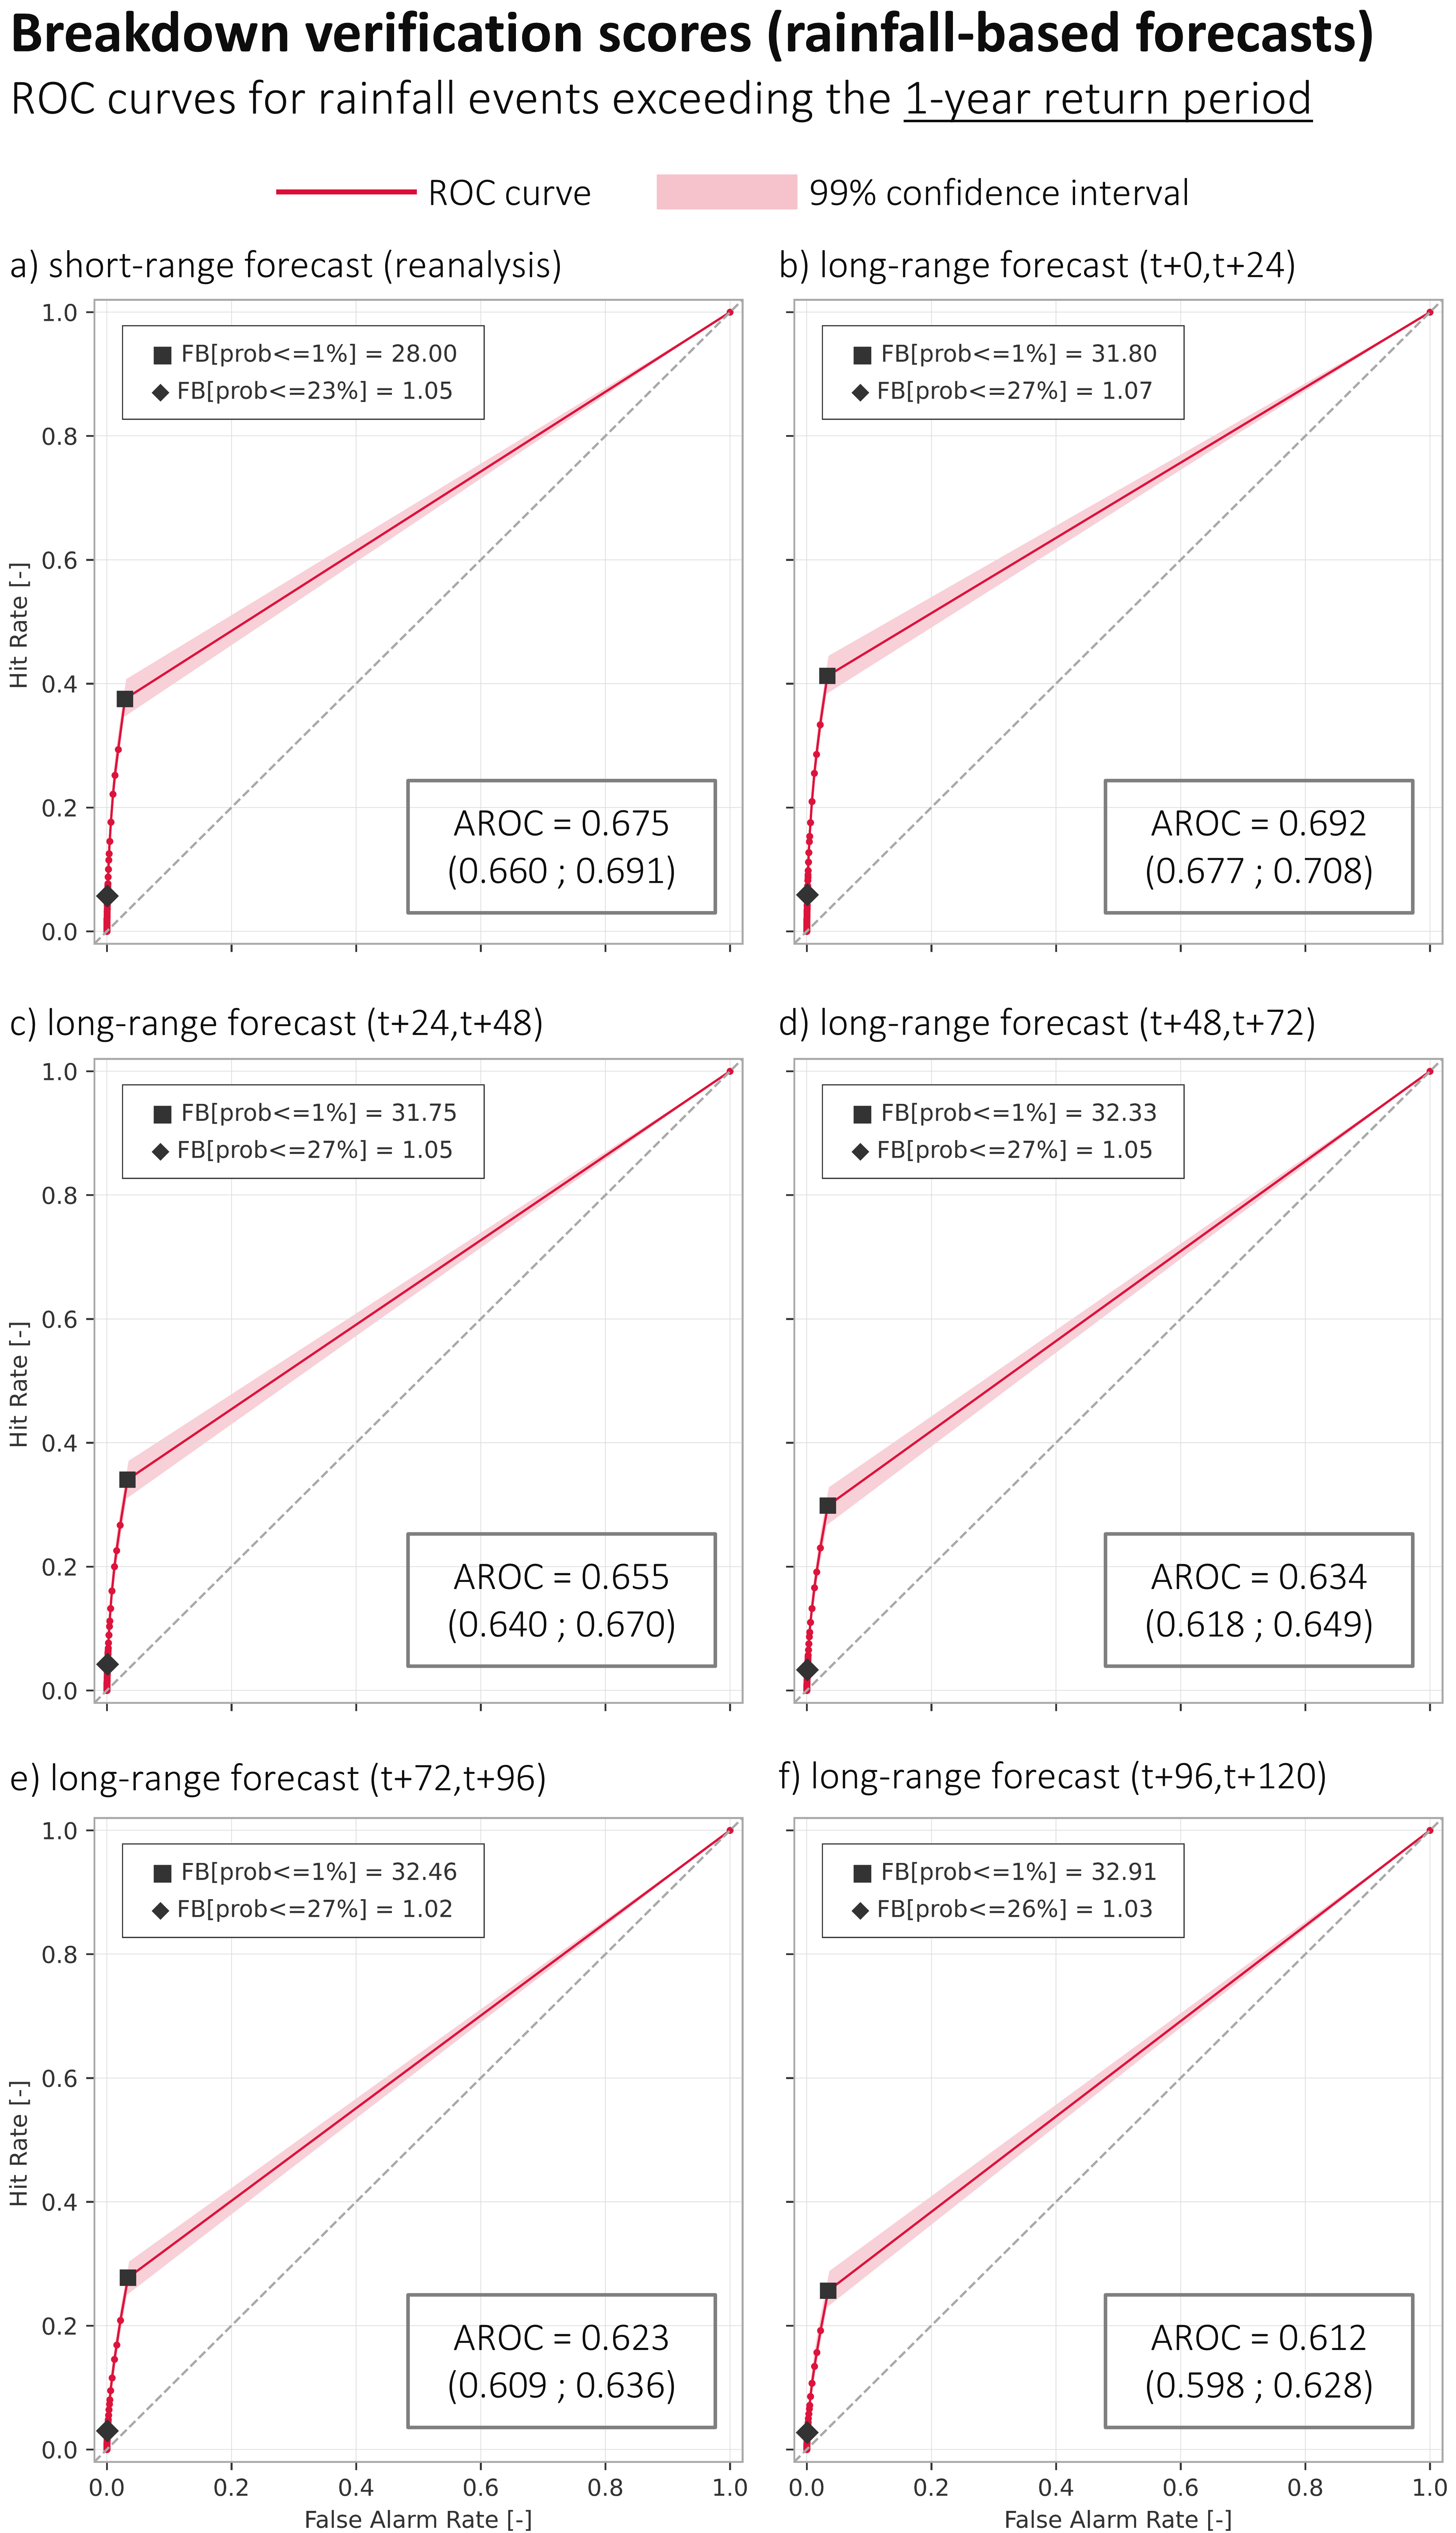
\includegraphics[width=\textwidth]{chapter_05/figures/rainfall_based_ff_verif_breakdown_scores_roc_1rp.png}
\caption{\textbf{ROC curves for tp >= 1-year return period for the rainfall-based forecasts of areas at risk of flash floods built with ERA5-ecPoint.} Panel (a) shows the ROC curve (blue solid line) for the short-range predictions together with the confidence intervals (blue shaded area) at 99\% confidence level. Panels (b) to (f) refer to the long-range forecasts, for accumulation periods ending in t+24, t+48, t+72, t+96, and t+120, respectively. The pink dots refer to the probability threshold at which the frequency bias has the closest value to 1 (i.e., perfectly reliable forecast), while the orange dot shows the value of the frequency bias for the lowest probability threshold available in ERA5-ecPoint (i.e., the 99th percentile).}
\label{fig:rainfall_based_ff_verif_breakdown_scores_roc_1rp}
\end{figure}

The pink dot in Figure \ref{fig:rainfall_based_ff_verif_breakdown_scores_roc_1rp}a shows that perfect reliability (i.e. frequency bias equal to 1) is reach for probabilities <= 23\%. For the long-range forecasts, the probability thresholds at which perfect reliability is achieved is compatible to the short-range, being 27\% for all the lead times except t+120 which is 26\%. The frequency bias for the lowest probability threshold (i.e. 99th percentile or probability threshold equal to 1\%) in the short-range forecasts equals to 28. The frequency biases for the long-range forecasts are similar, falling between 31 and 33. 

Similar results are obtained for the 5-, 10-, 20-, 50-, and 100-year return periods.

\begin{figure}[htbp]
\centering
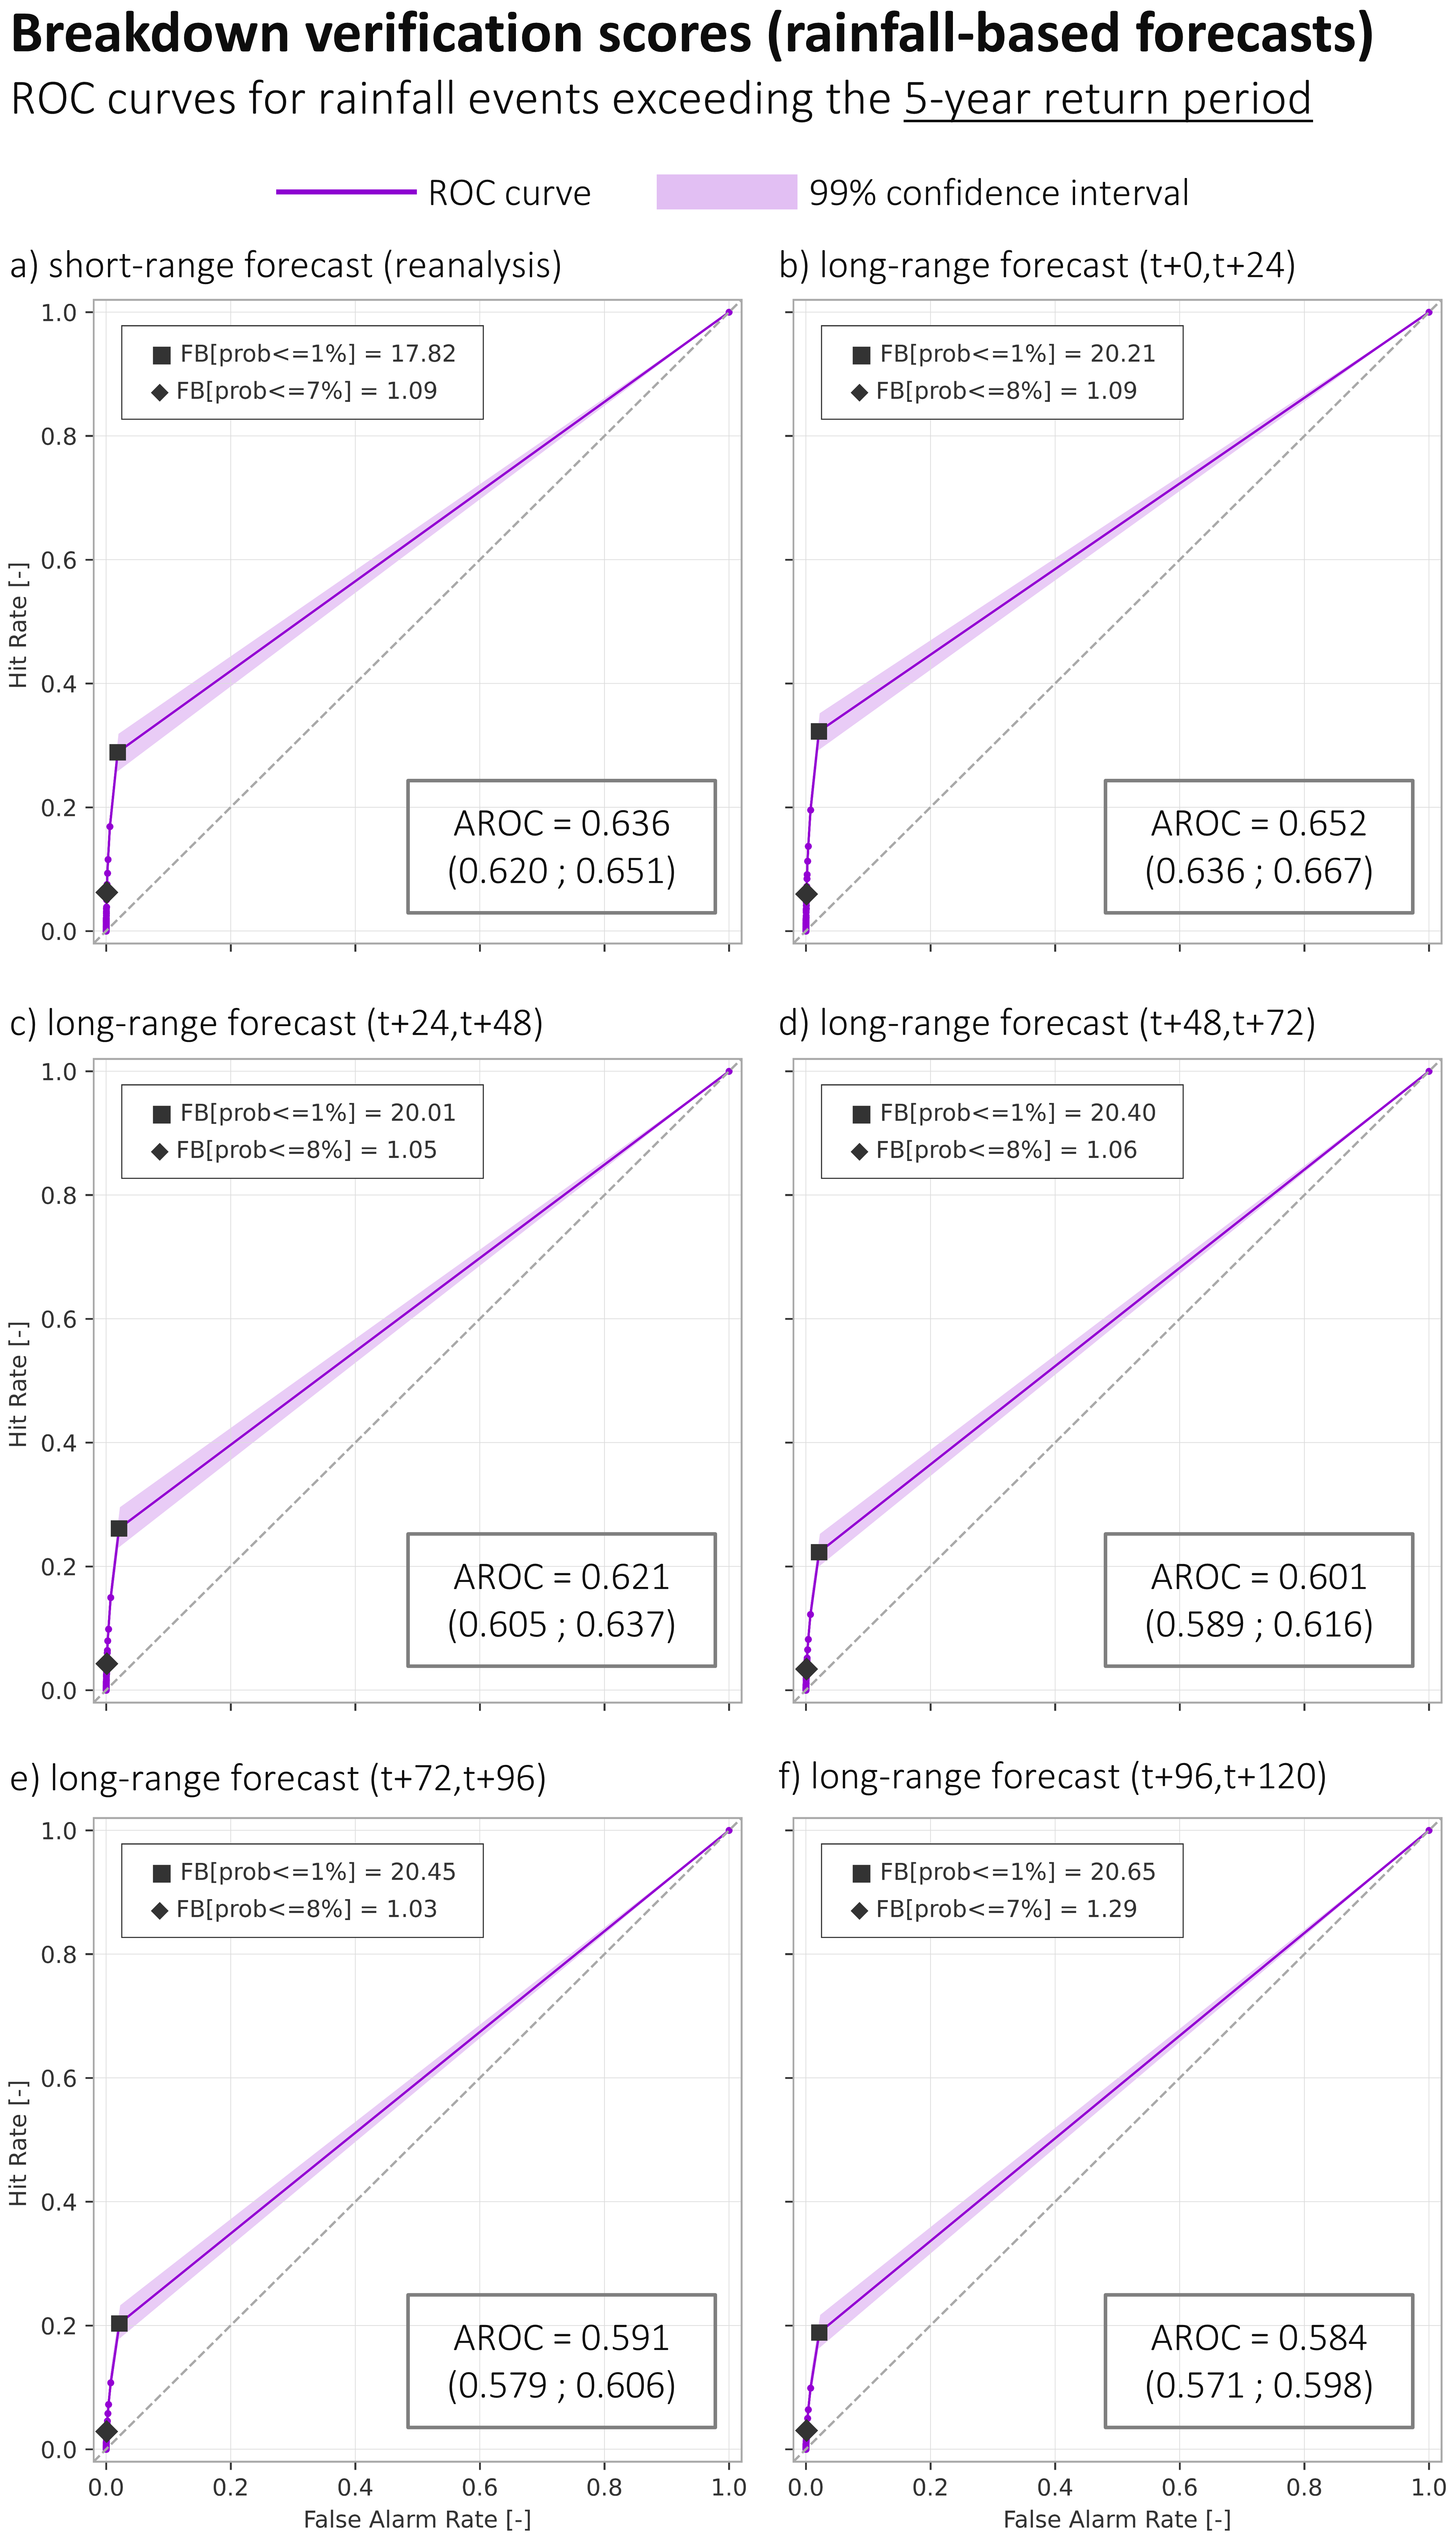
\includegraphics[width=\textwidth]{chapter_05/figures/rainfall_based_ff_verif_breakdown_scores_roc_5rp.png}
\caption{\textbf{ROC curves for tp >= 5-year return period for the rainfall-based forecasts of areas at risk of flash floods built with ERA5-ecPoint.} Similar to Figure \ref{fig:rainfall_based_ff_verif_breakdown_scores_roc_1rp}.}
\label{fig:rainfall_based_ff_verif_breakdown_scores_roc_5rp}
\end{figure}

\begin{figure}[htbp]
\centering
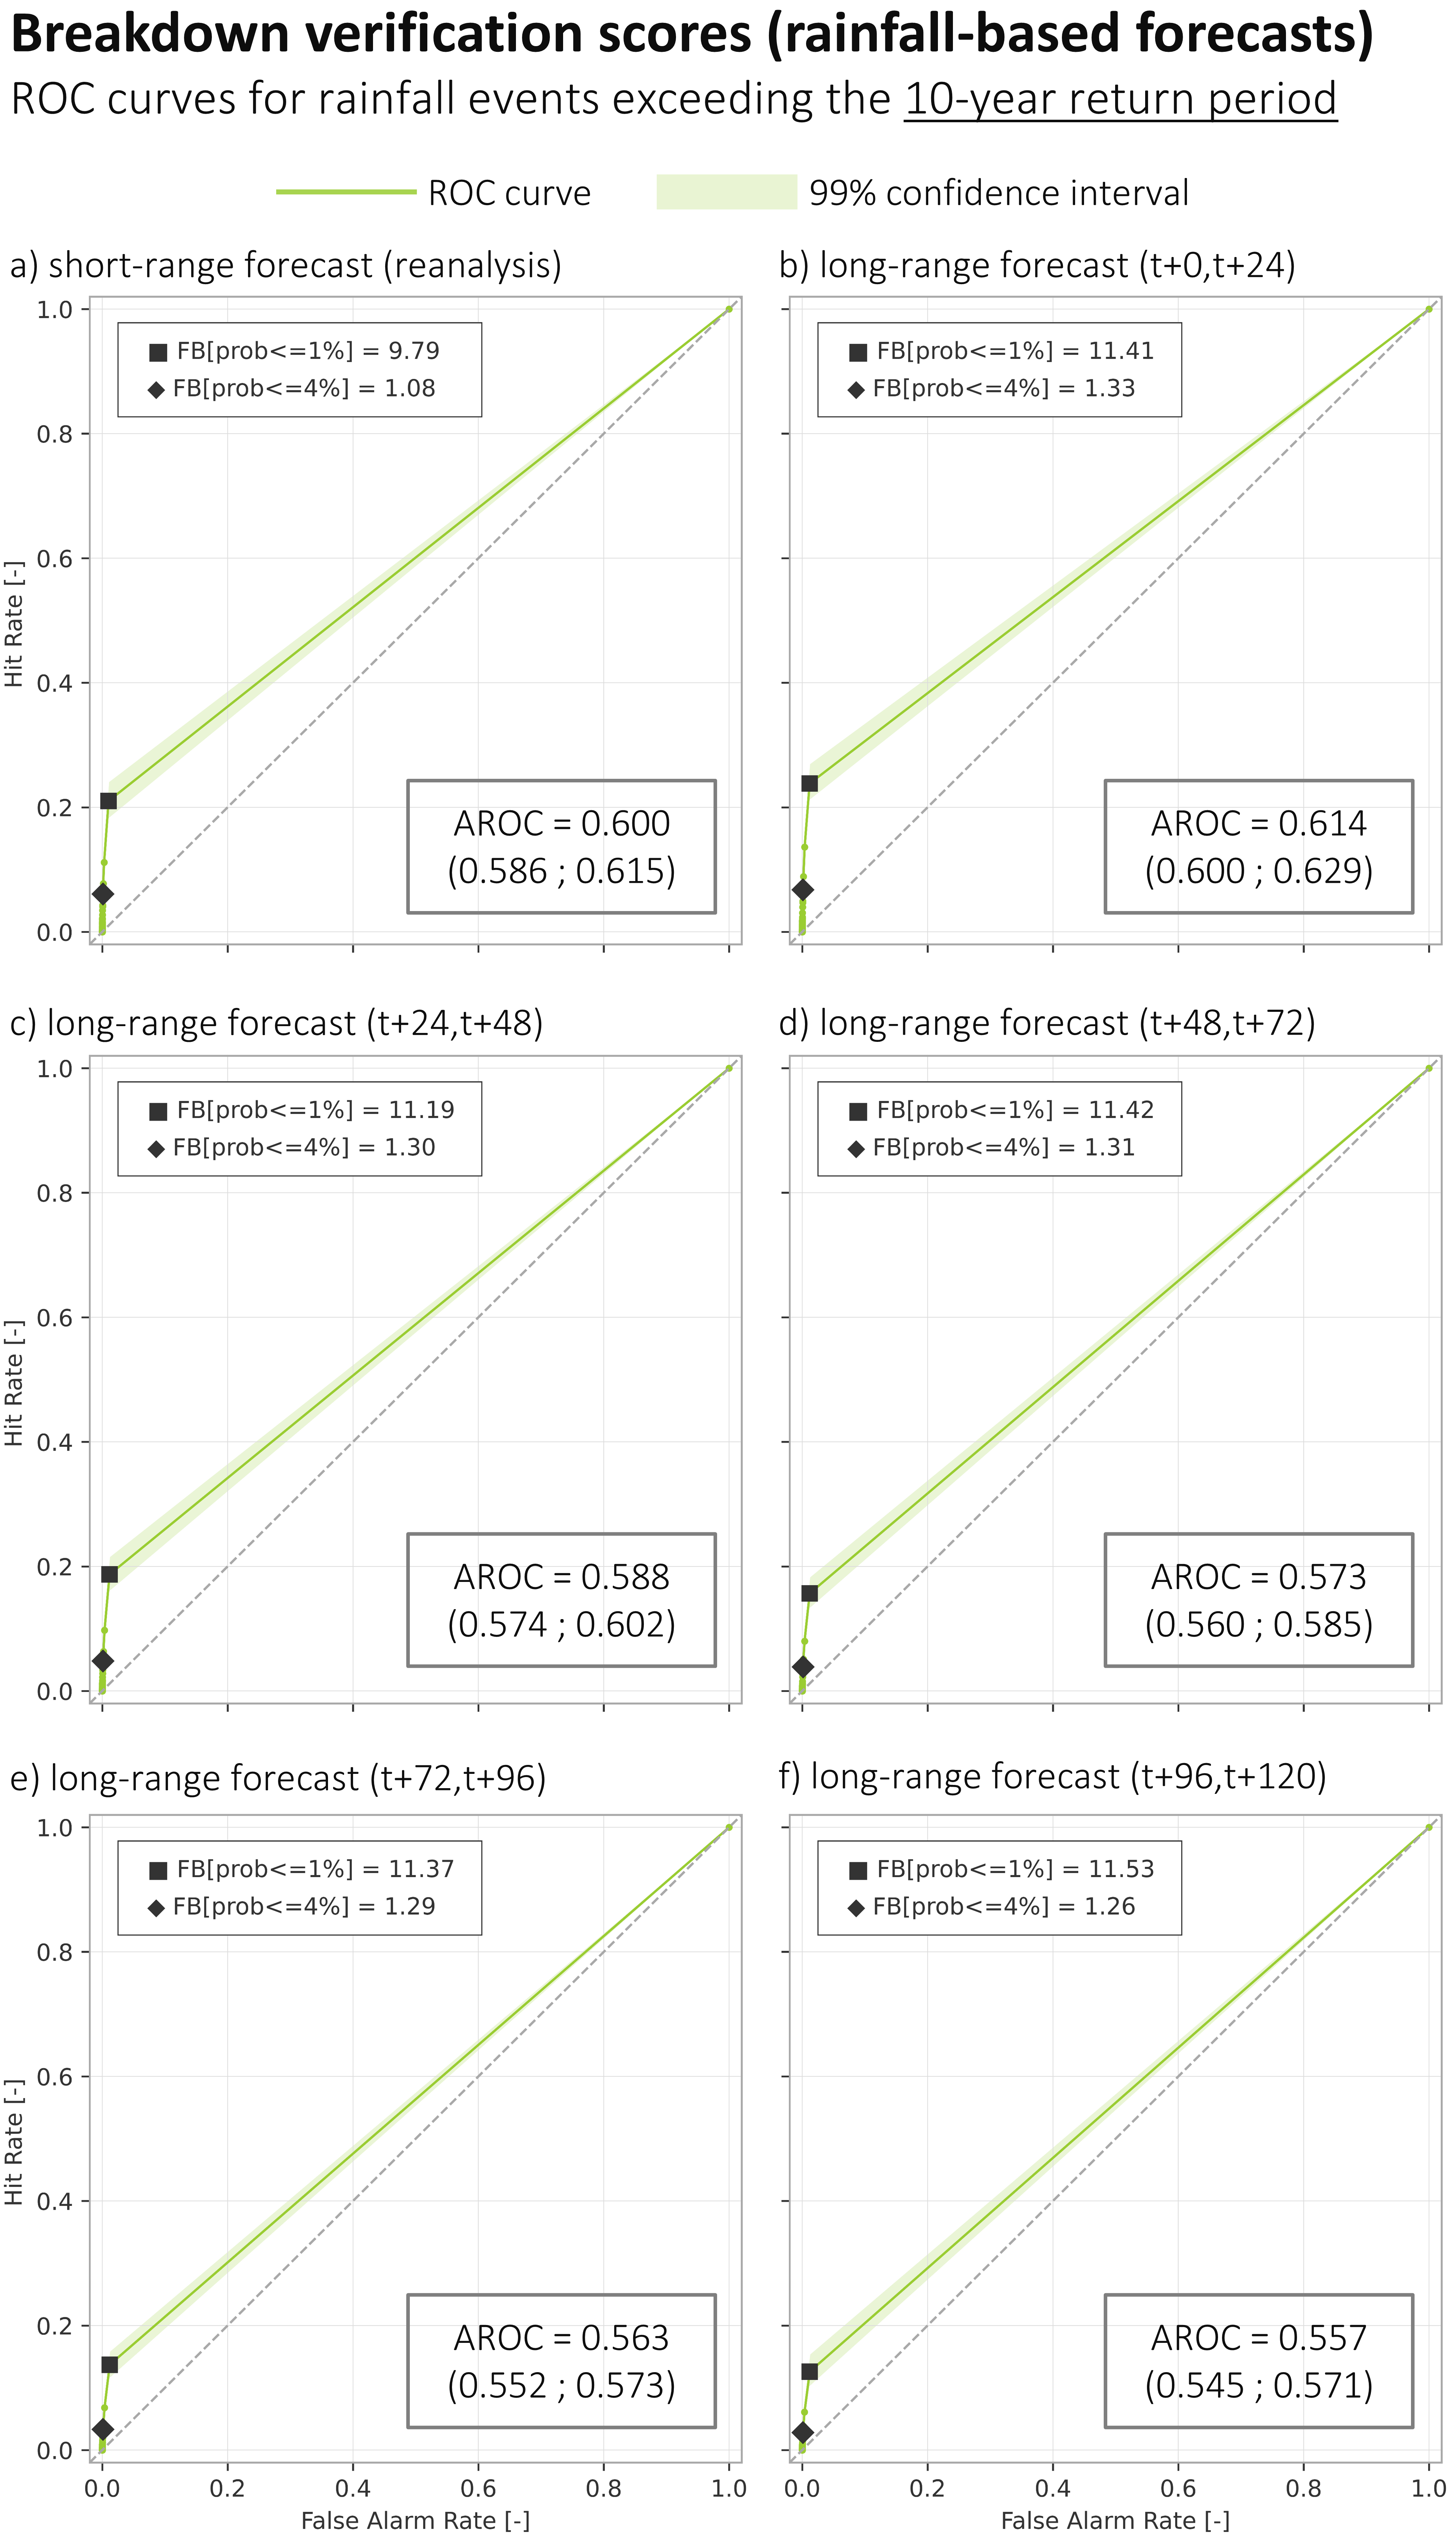
\includegraphics[width=\textwidth]{chapter_05/figures/rainfall_based_ff_verif_breakdown_scores_roc_10rp.png}
\caption{\textbf{ROC curves for tp >= 10-year return period for the rainfall-based forecasts of areas at risk of flash floods built with ERA5-ecPoint.} Similar to Figure \ref{fig:rainfall_based_ff_verif_breakdown_scores_roc_1rp}.}
\label{fig:rainfall_based_ff_verif_breakdown_scores_roc_10rp}
\end{figure}

\begin{figure}[htbp]
\centering
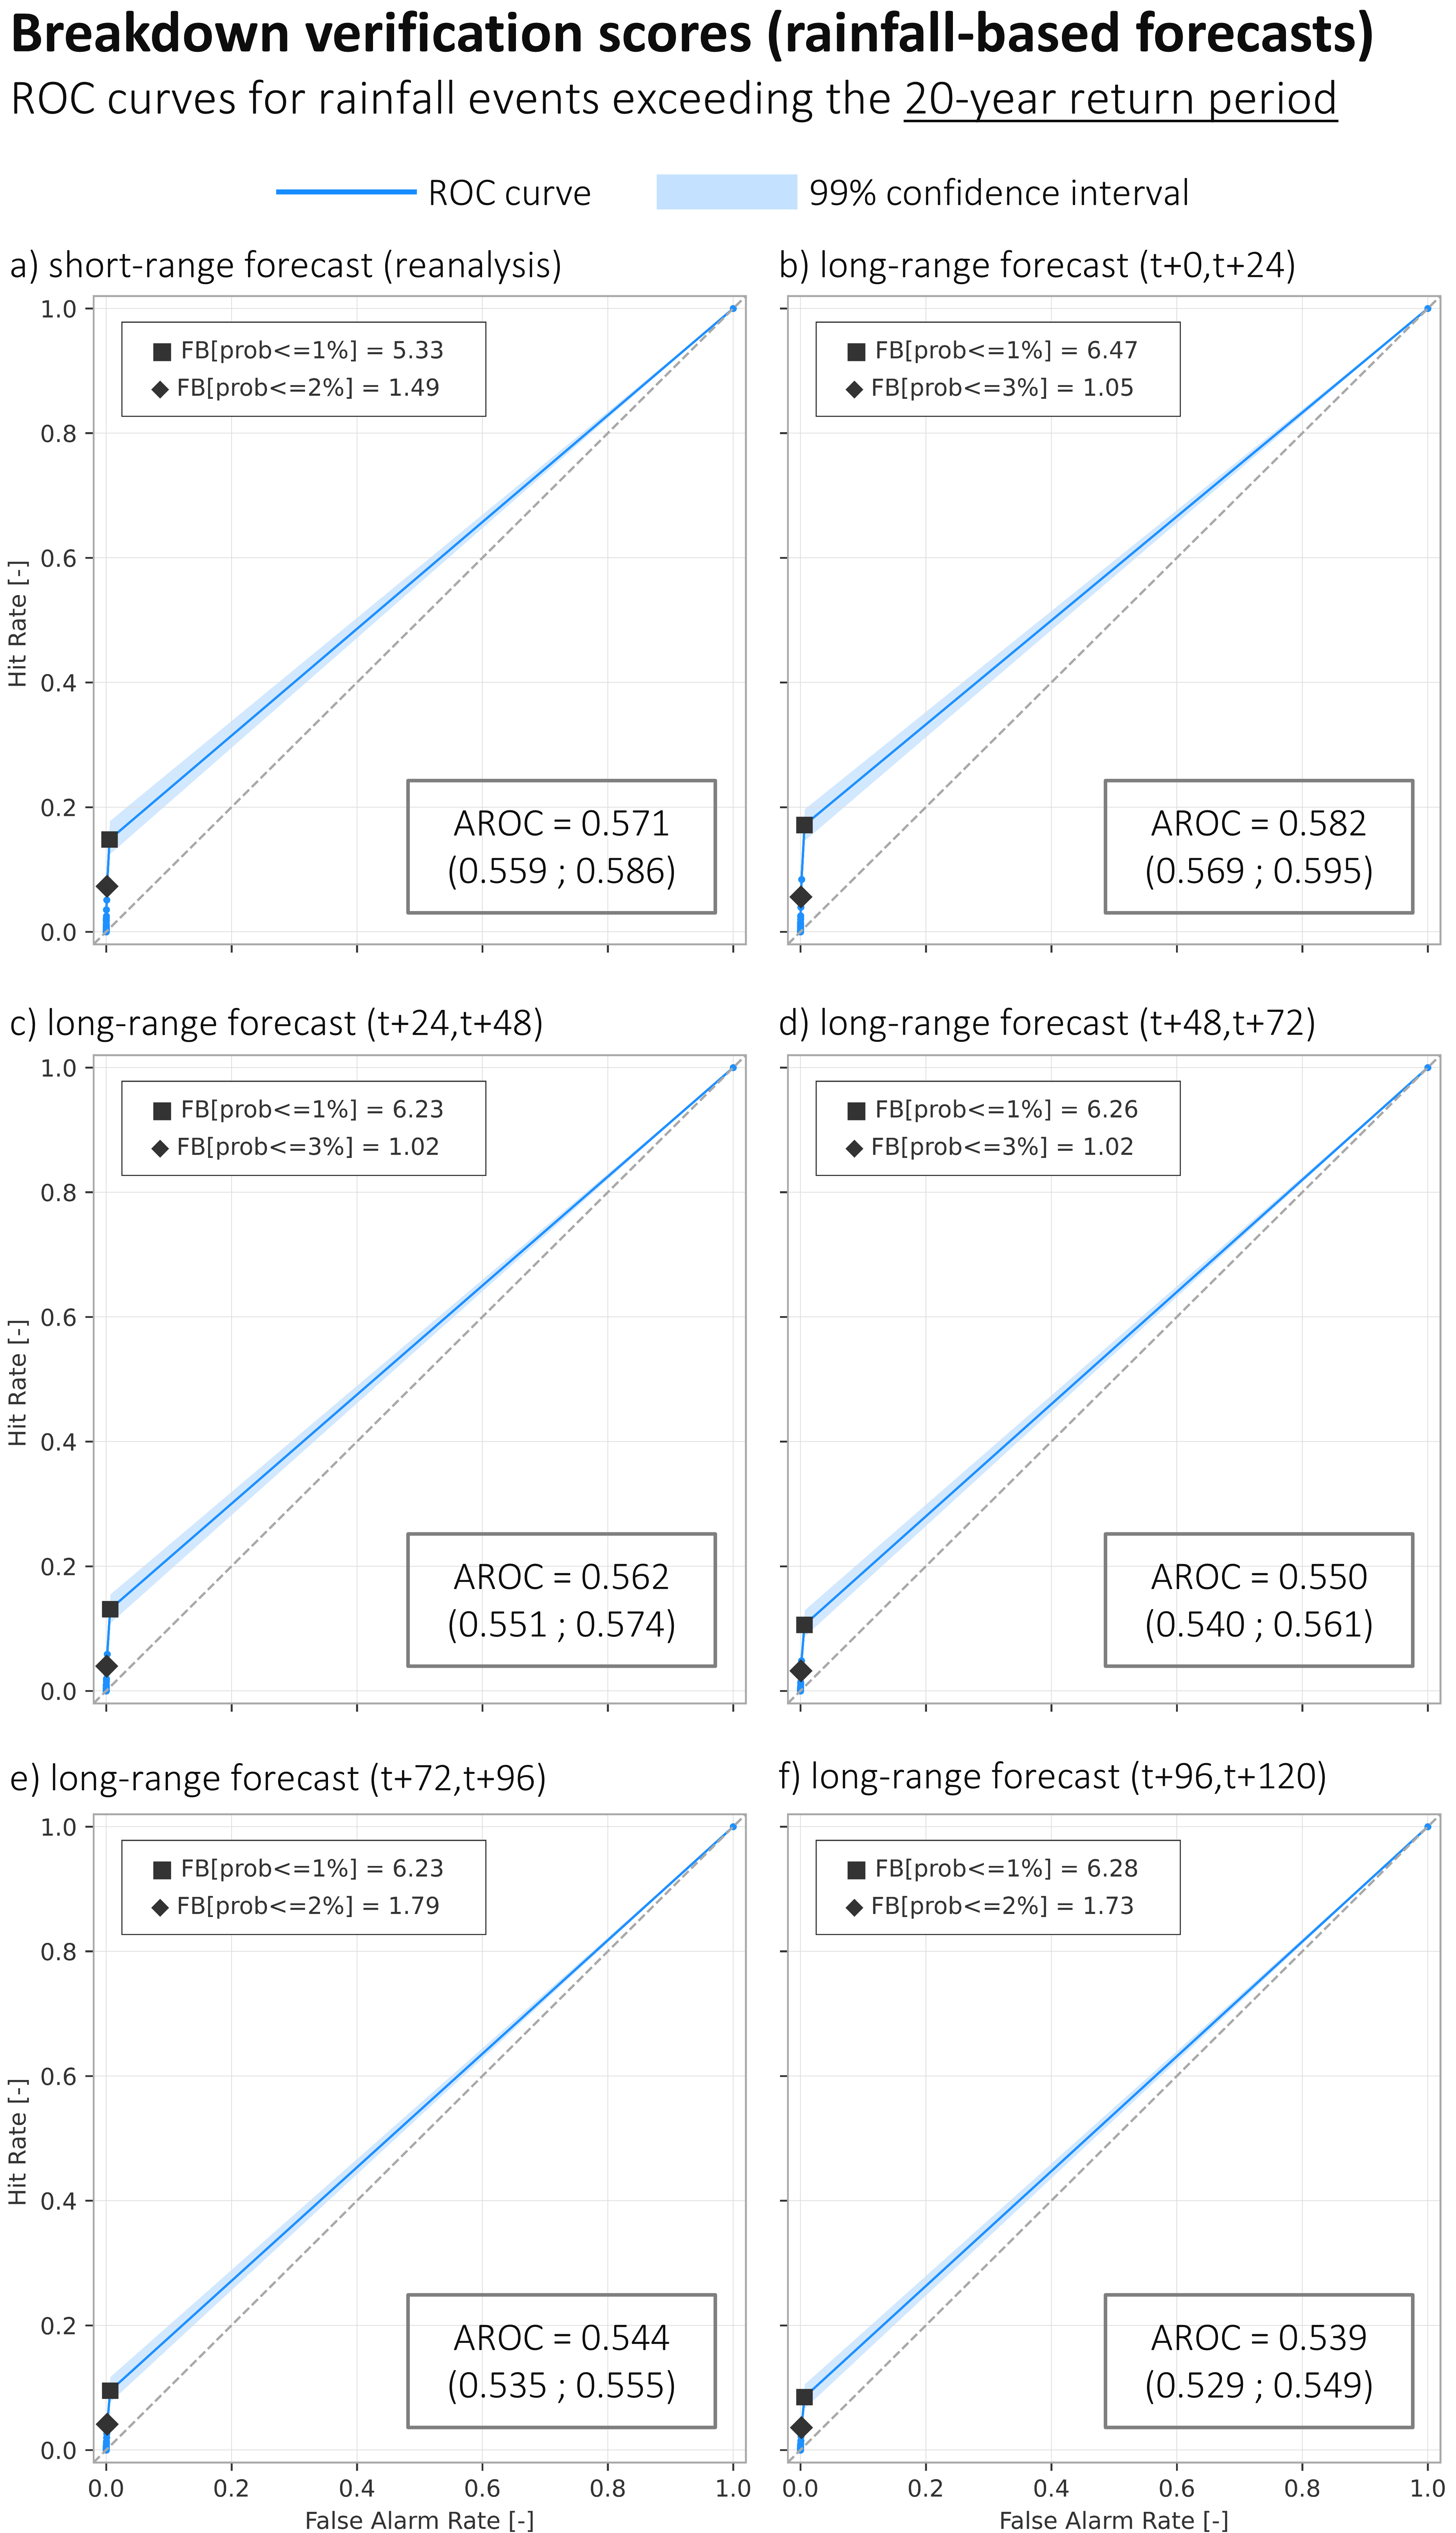
\includegraphics[width=\textwidth]{chapter_05/figures/rainfall_based_ff_verif_breakdown_scores_roc_20rp.png}
\caption{\textbf{ROC curves for tp >= 20-year return period for the rainfall-based forecasts of areas at risk of flash floods built with ERA5-ecPoint.} Similar to Figure \ref{fig:rainfall_based_ff_verif_breakdown_scores_roc_1rp}.}
\label{fig:rainfall_based_ff_verif_breakdown_scores_roc_20rp}
\end{figure}

\begin{figure}[htbp]
\centering
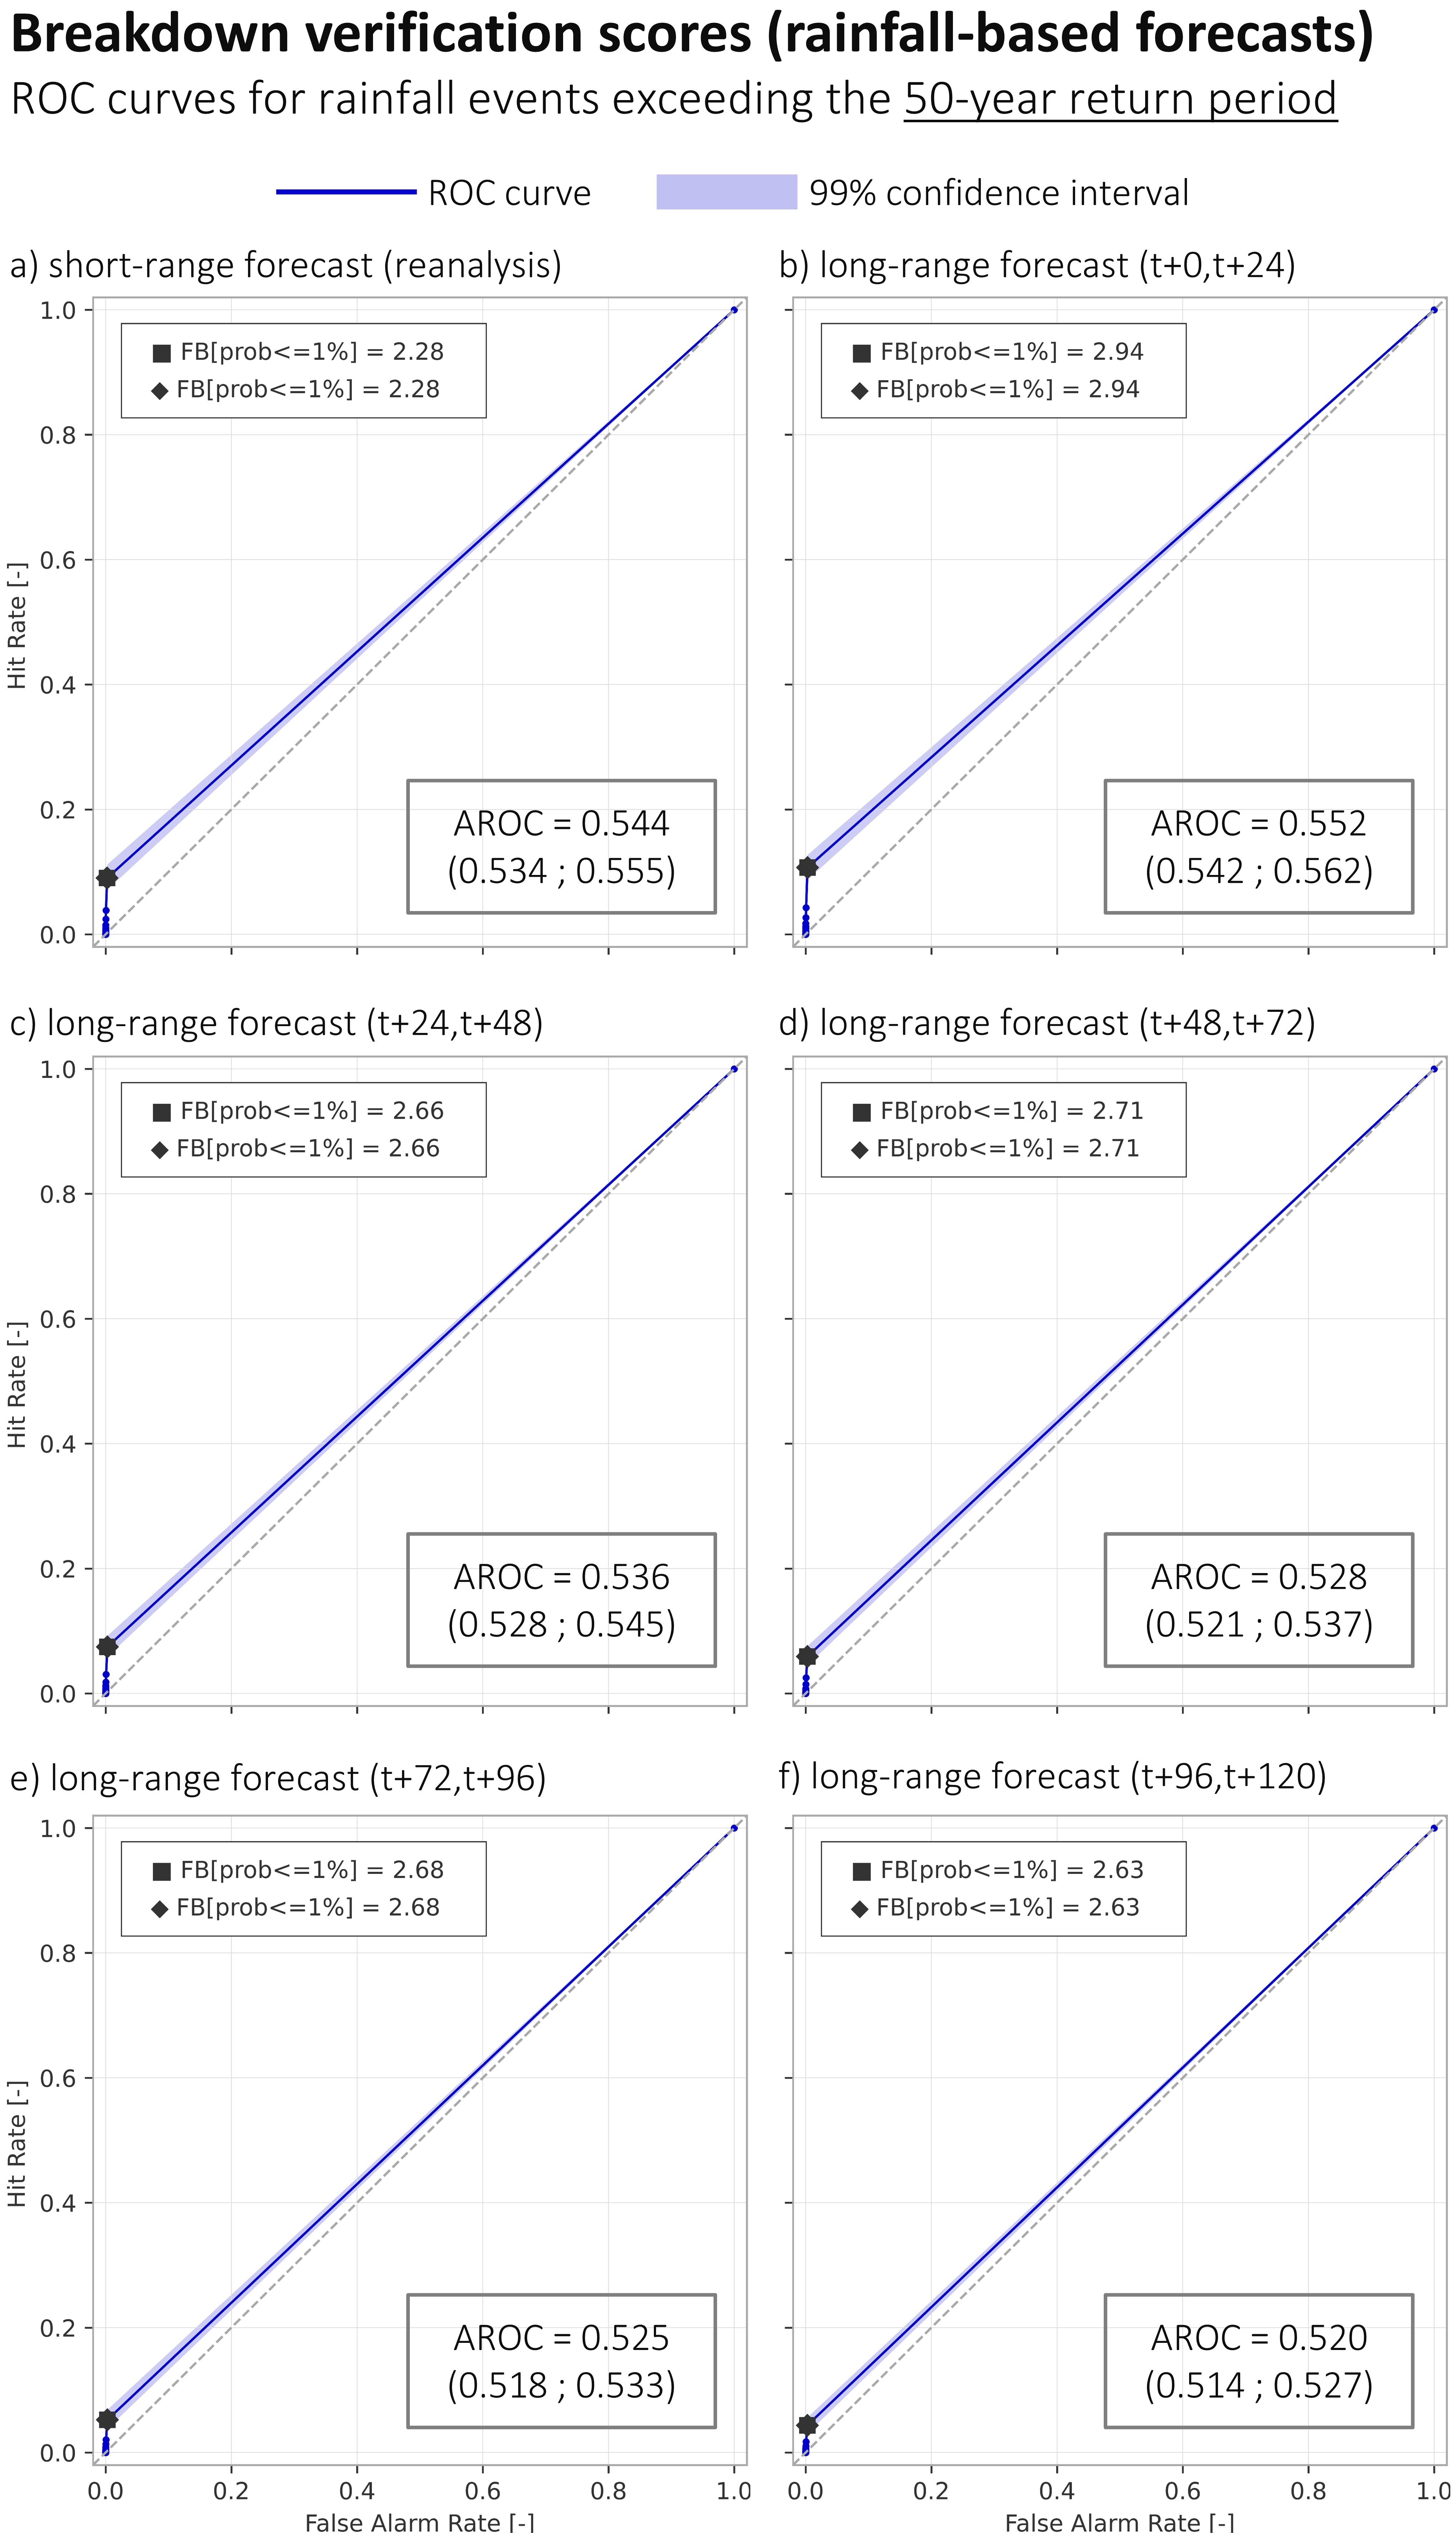
\includegraphics[width=\textwidth]{chapter_05/figures/rainfall_based_ff_verif_breakdown_scores_roc_50rp.png}
\caption{\textbf{ROC curves for tp >= 50-year return period for the rainfall-based forecasts of areas at risk of flash floods built with ERA5-ecPoint.} Similar to Figure \ref{fig:rainfall_based_ff_verif_breakdown_scores_roc_1rp}.}
\label{fig:rainfall_based_ff_verif_breakdown_scores_roc_50rp}
\end{figure}

\begin{figure}[htbp]
\centering
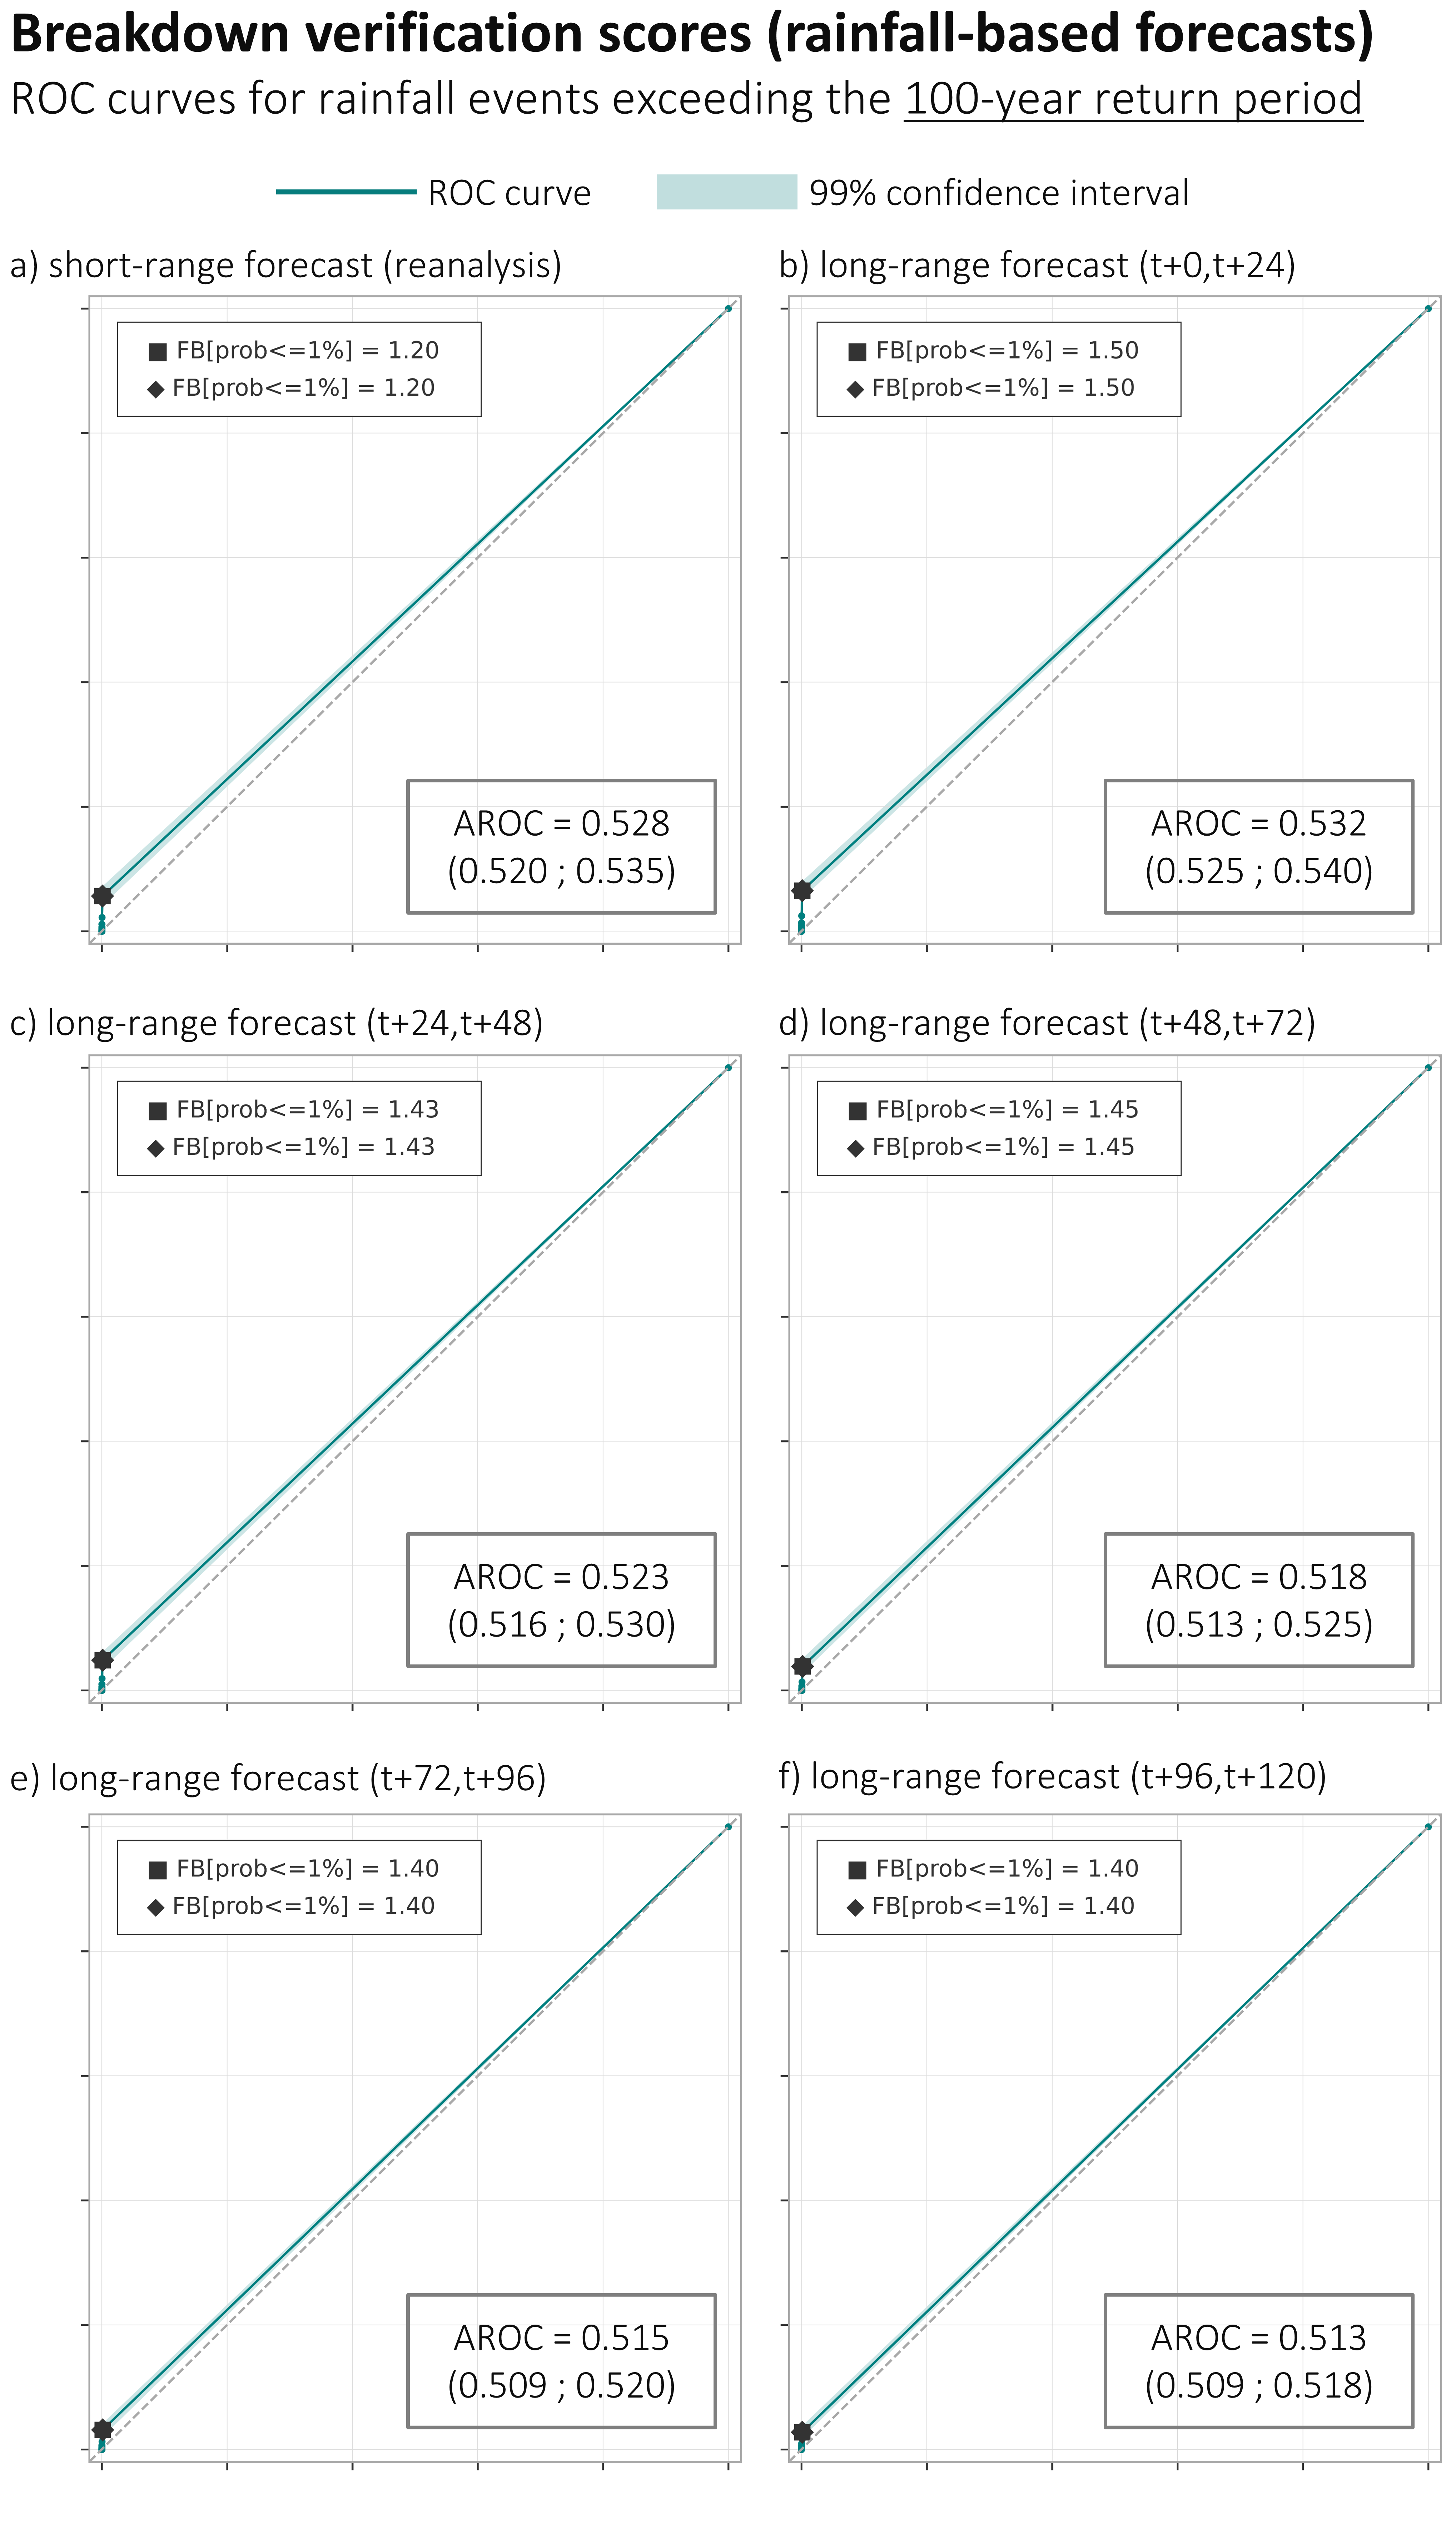
\includegraphics[width=\textwidth]{chapter_05/figures/rainfall_based_ff_verif_breakdown_scores_roc_100rp.png}
\caption{\textbf{ROC curves for tp >= 100-year return period for the rainfall-based forecasts of areas at risk of flash floods built with ERA5-ecPoint.} Similar to Figure \ref{fig:rainfall_based_ff_verif_breakdown_scores_roc_1rp}.}
\label{fig:rainfall_based_ff_verif_breakdown_scores_roc_100rp}
\end{figure}


\subsection{Reliability}

All forecasts for rainfall events exceeding the 1-year return period threshold (Figure \ref{fig:rainfall_based_ff_verif_breakdown_scores_rel_diag_1rp}) exhibit a systematic overprediction across all lead times, as shown by the reliability diagram being below the diagonal line. This indicates that when the model predicts a given probability, the observed frequency of flash flood events is consistently lower. For example, when the forecasts indicate a 50\% chance of having a flash flood event, the observed frequency ranges from \sim10\% in the short-range forecasts (Figure \ref{fig:rainfall_based_ff_verif_breakdown_scores_rel_diag_1rp}a), and between 10\% (for t+24, Figure \ref{fig:rainfall_based_ff_verif_breakdown_scores_rel_diag_1rp}b) and 2\% (t+120, Figure \ref{fig:rainfall_based_ff_verif_breakdown_scores_rel_diag_1rp}f) in the long-range forecasts. As seen in the ROC curves, the confidence intervals at 99\% are fairly narrow, suggesting that the differences between the reliability diagrams at different lead times are significant at the considered confidence level. However, the confidence levels increase with increasing forecast probabilities. As seen in the corresponding sharpness diagrams (inset boxes in all panels of Figure \ref{fig:rainfall_based_ff_verif_breakdown_scores_rel_diag_1rp}), such widening of the confidence intervals is likely due to the low number of forecasts issued with probabilities higher than ~25\% (when the total number of instances lies below 1000 samples). Such predominance of low probability forecasts suggests that the model (ERA5-ecPoint) rarely expresses high confidence in extreme event occurrence. A notable characteristic of all the reliability diagrams in the Figure \ref{fig:rainfall_based_ff_verif_breakdown_scores_rel_diag_1rp} is the sharp increase in observed frequency for the highest probability bins (i.e. 80\% to 100\%). This steep rise suggests that when the model does issue high probability forecasts, these correspond to genuinely extreme events, though such forecasts remain infrequent.

\begin{figure}[htbp]
\centering
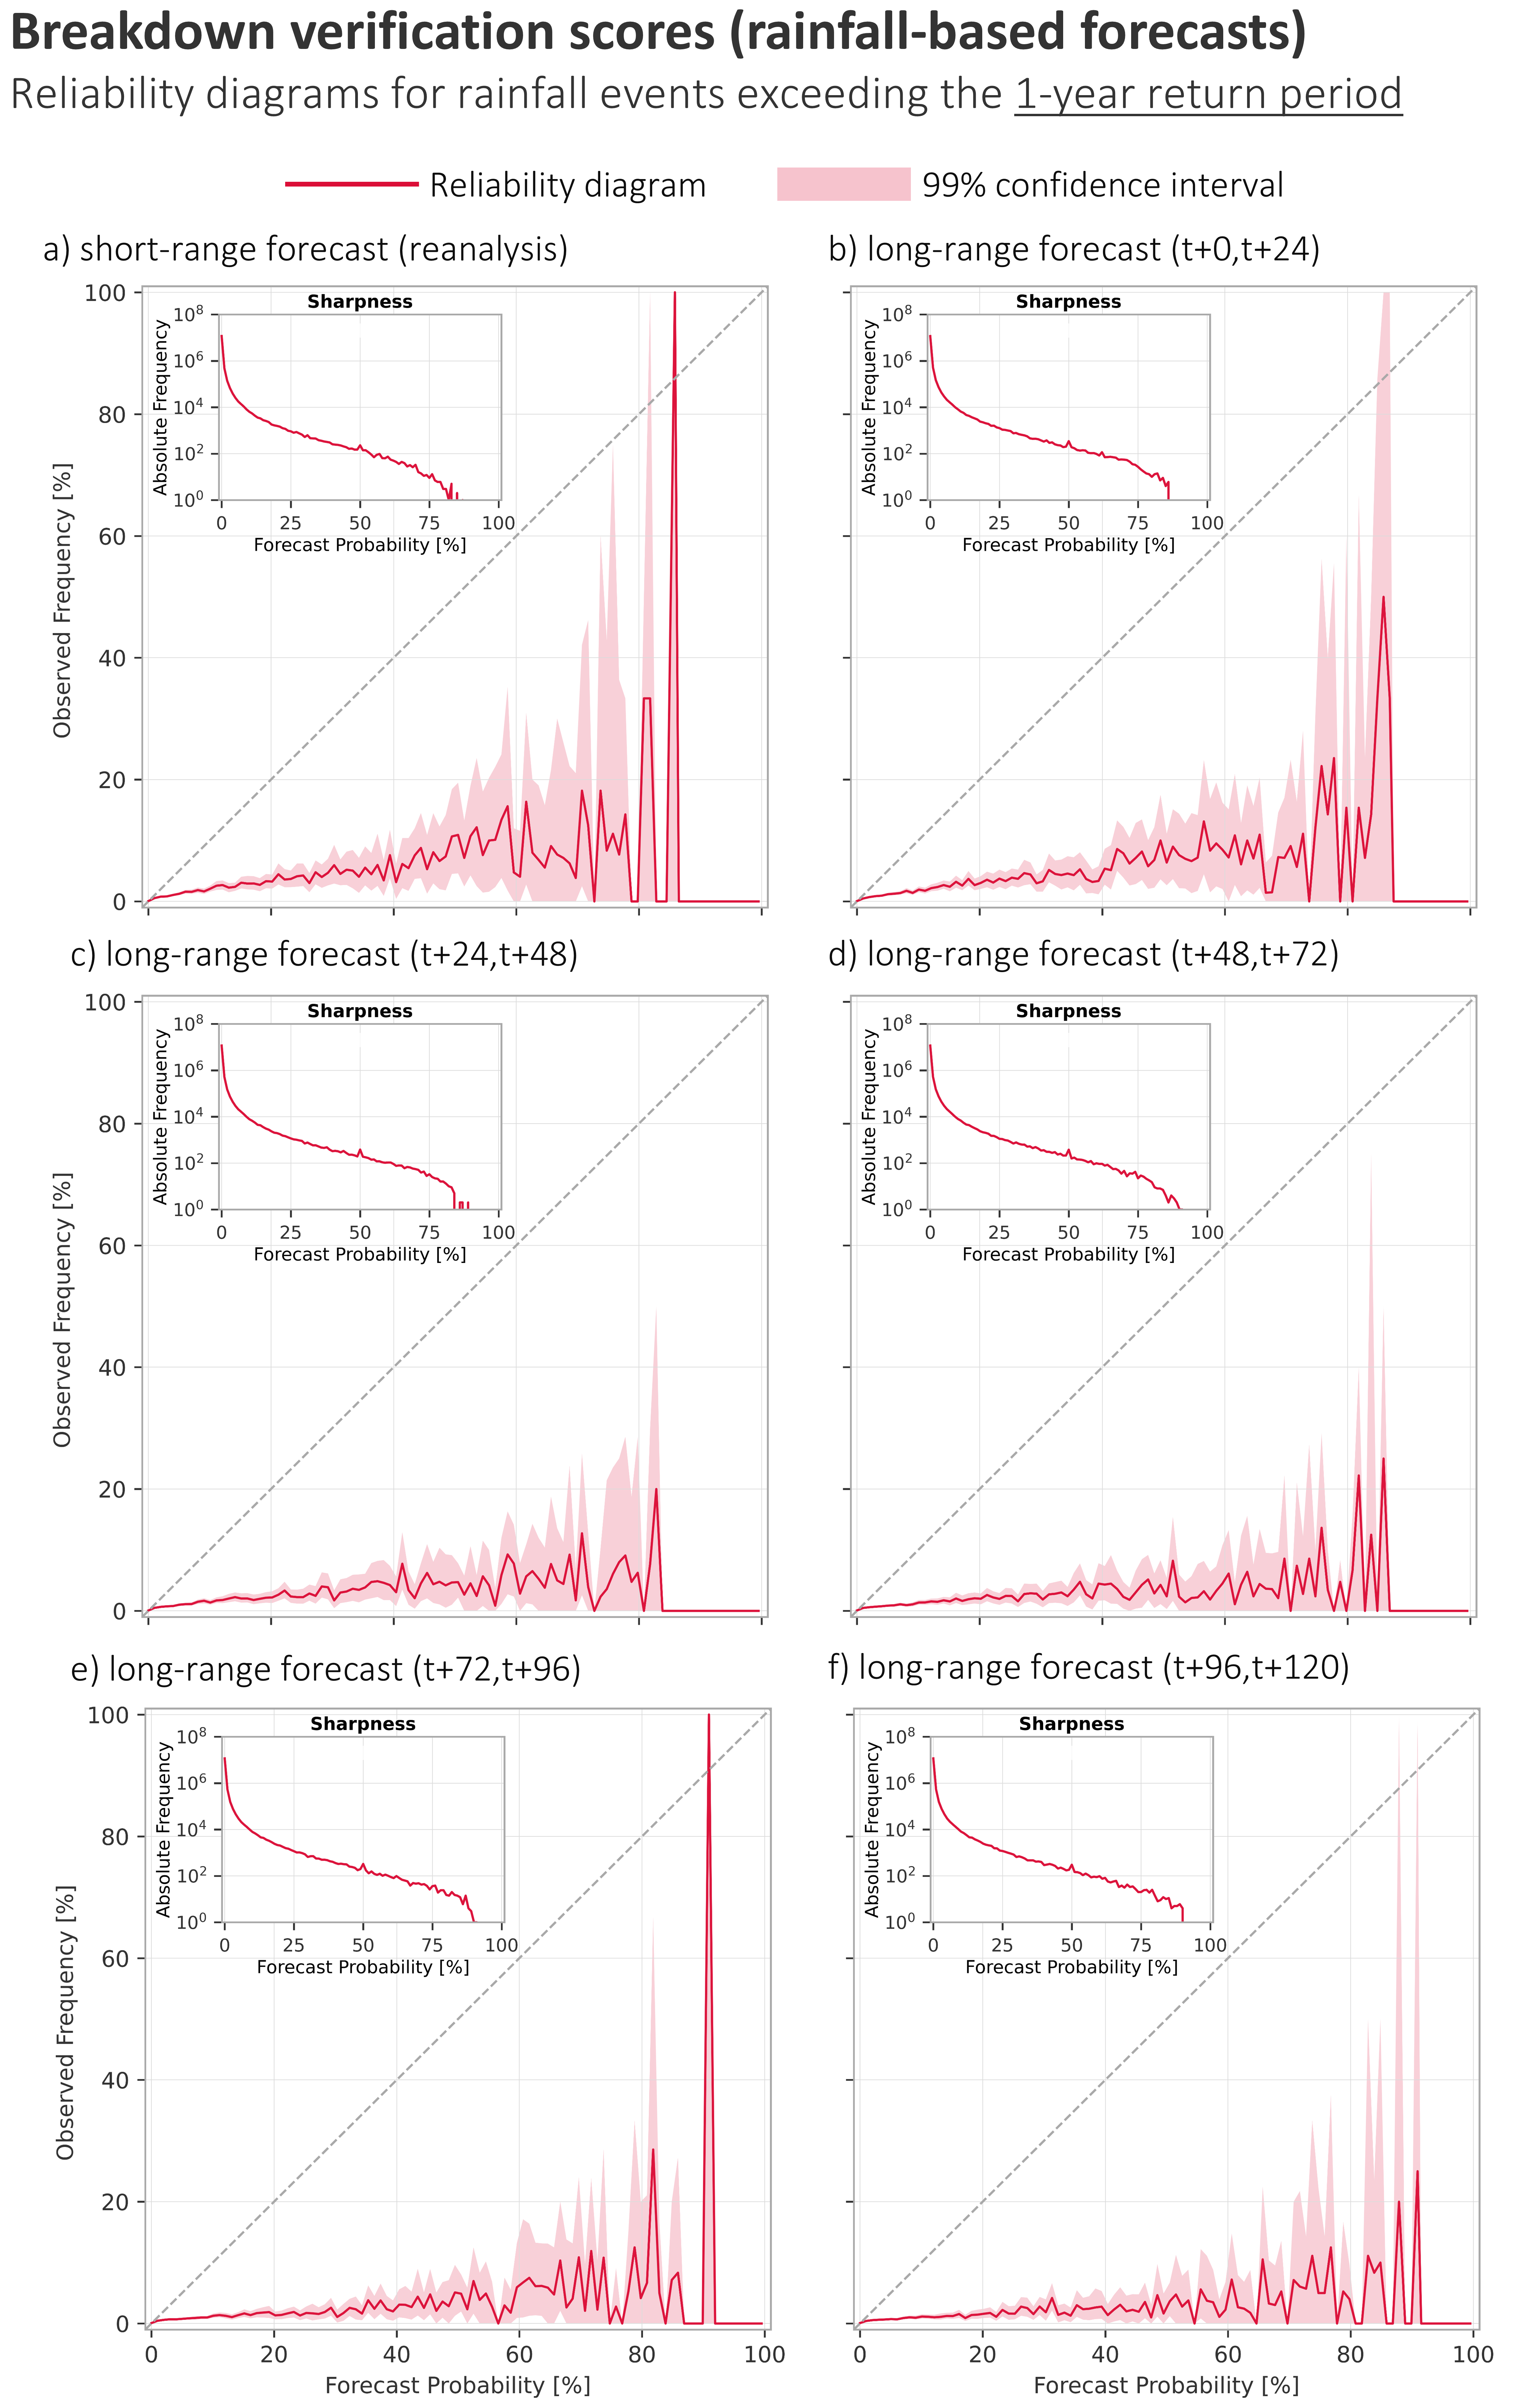
\includegraphics[width=\textwidth]{rainfall_based_ff_verif_breakdown_scores_rel_diag_1rp.png}
\caption{\textbf{Reliability diagrams for tp >= 1-year return period for the rainfall-based forecasts of areas at risk of flash floods built with ERA5-ecPoint.} Panel (a) shows the reliability diagram (blue solid line) for the short-range predictions together with the confidence intervals (blue shaded area) at 99\% confidence level. Panels (b) to (f) refer to the long-range forecasts for accumulation periods ending in t+24, t+48, t+72, t+96, and t+120, respectively. The inset boxes show the corresponding sharpness diagrams.}
\label{fig:rainfall_based_ff_verif_breakdown_scores_rel_diag_1rp}
\end{figure}

The temporal evolution from Figure \ref{fig:rainfall_based_ff_verif_breakdown_scores_rel_diag_1rp}a to f reveals subtle changes in the forecasts' reliability characteristics with increasing lead time. Whilst the general pattern of overprediction persists, from day 2 forecasts (t+48) results more squashed into a flat line over very small observed frequencies, indicating that even though the model issues forecasts with high probabilities of exceeding the 1-year return period at longer lead times with a similar frequency of the short-range forecasts and the day 1 (t+24) long-range forecast, such forecasts do not necessarily correspond to an observed flash flood event.

The reliability diagrams get closer to the diagonal line (indicating perfect bias) as we increase the rainfall threshold to identify the flash flood events. Perfect reliability is observed for rainfall events exceeding the 10-, 20-year, and 50-year return period with probabilities below 5\% at day 1 forecast (t+24) for the 10-, 20-year return period, and 10\% for the 50-year return period.

\begin{figure}[htbp]
\centering
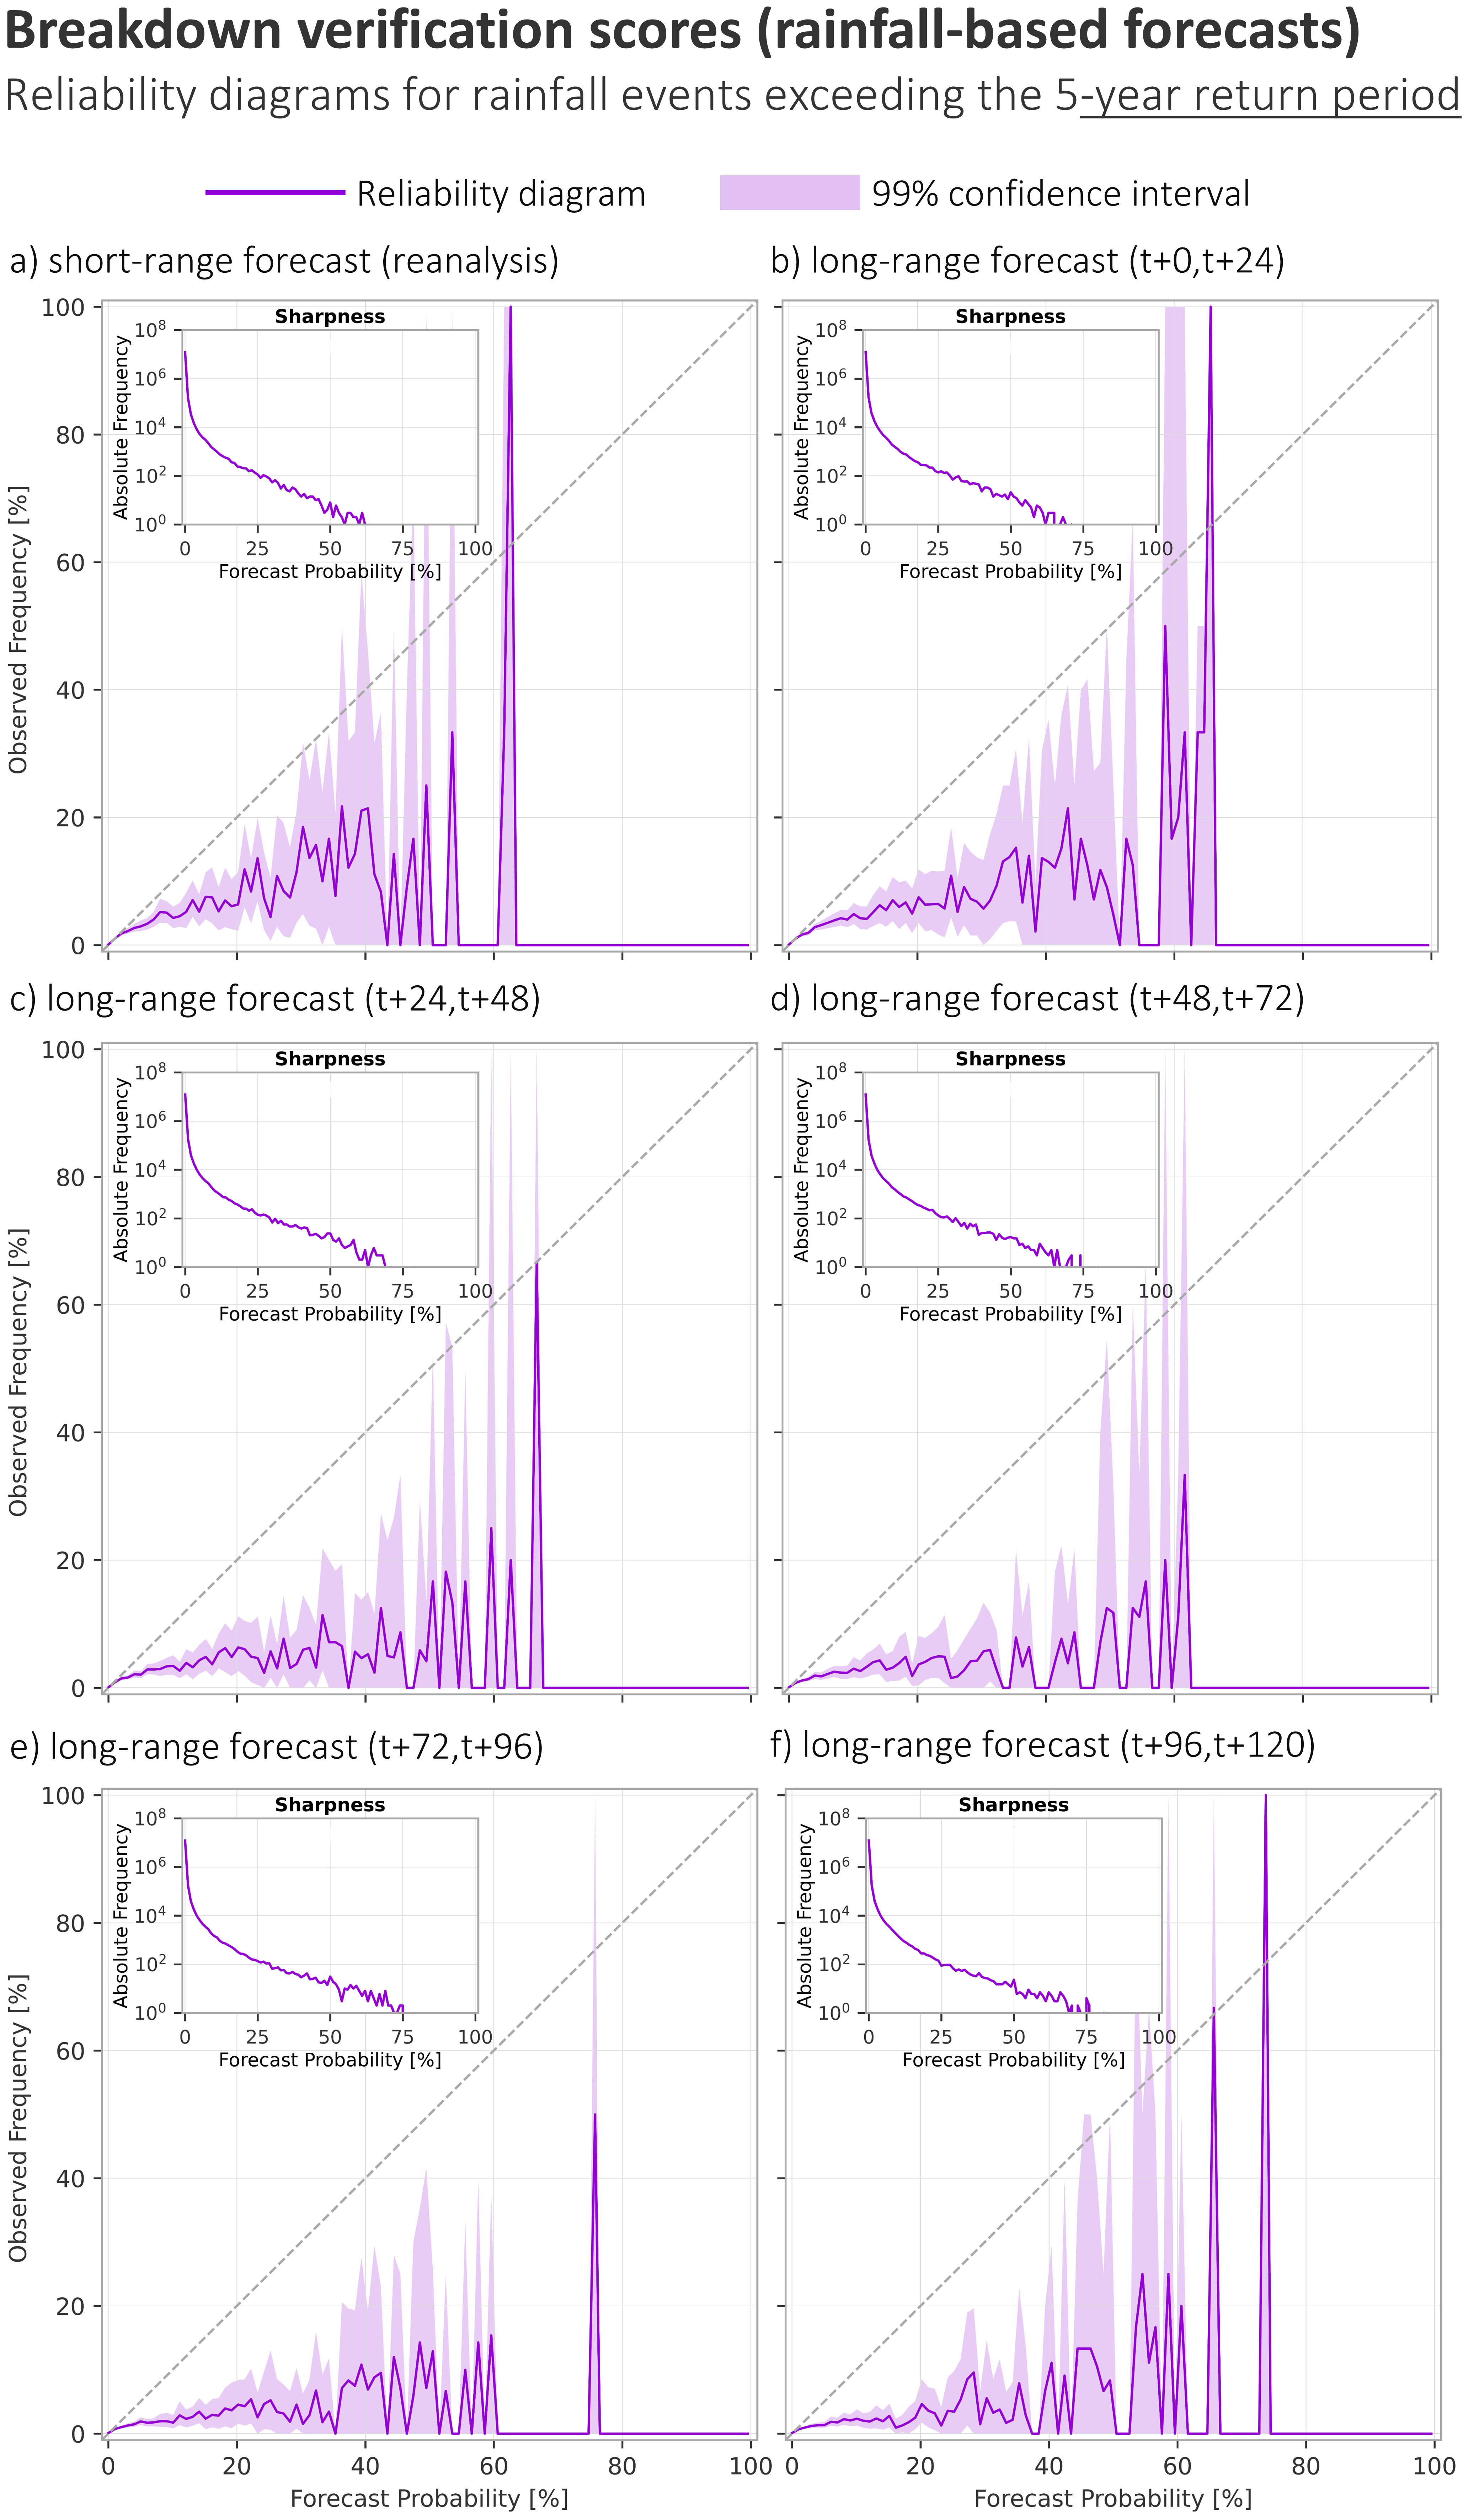
\includegraphics[width=\textwidth]{rainfall_based_ff_verif_breakdown_scores_rel_diag_5rp.png}
\caption{\textbf{Reliability diagrams for tp >= 5-year return period for the rainfall-based forecasts of areas at risk of flash floods built with ERA5-ecPoint.} Similar to Figure \ref{fig:rainfall_based_ff_verif_breakdown_scores_rel_diag_1rp}.}
\label{fig:rainfall_based_ff_verif_breakdown_scores_rel_diag_5rp}
\end{figure}

\begin{figure}[htbp]
\centering
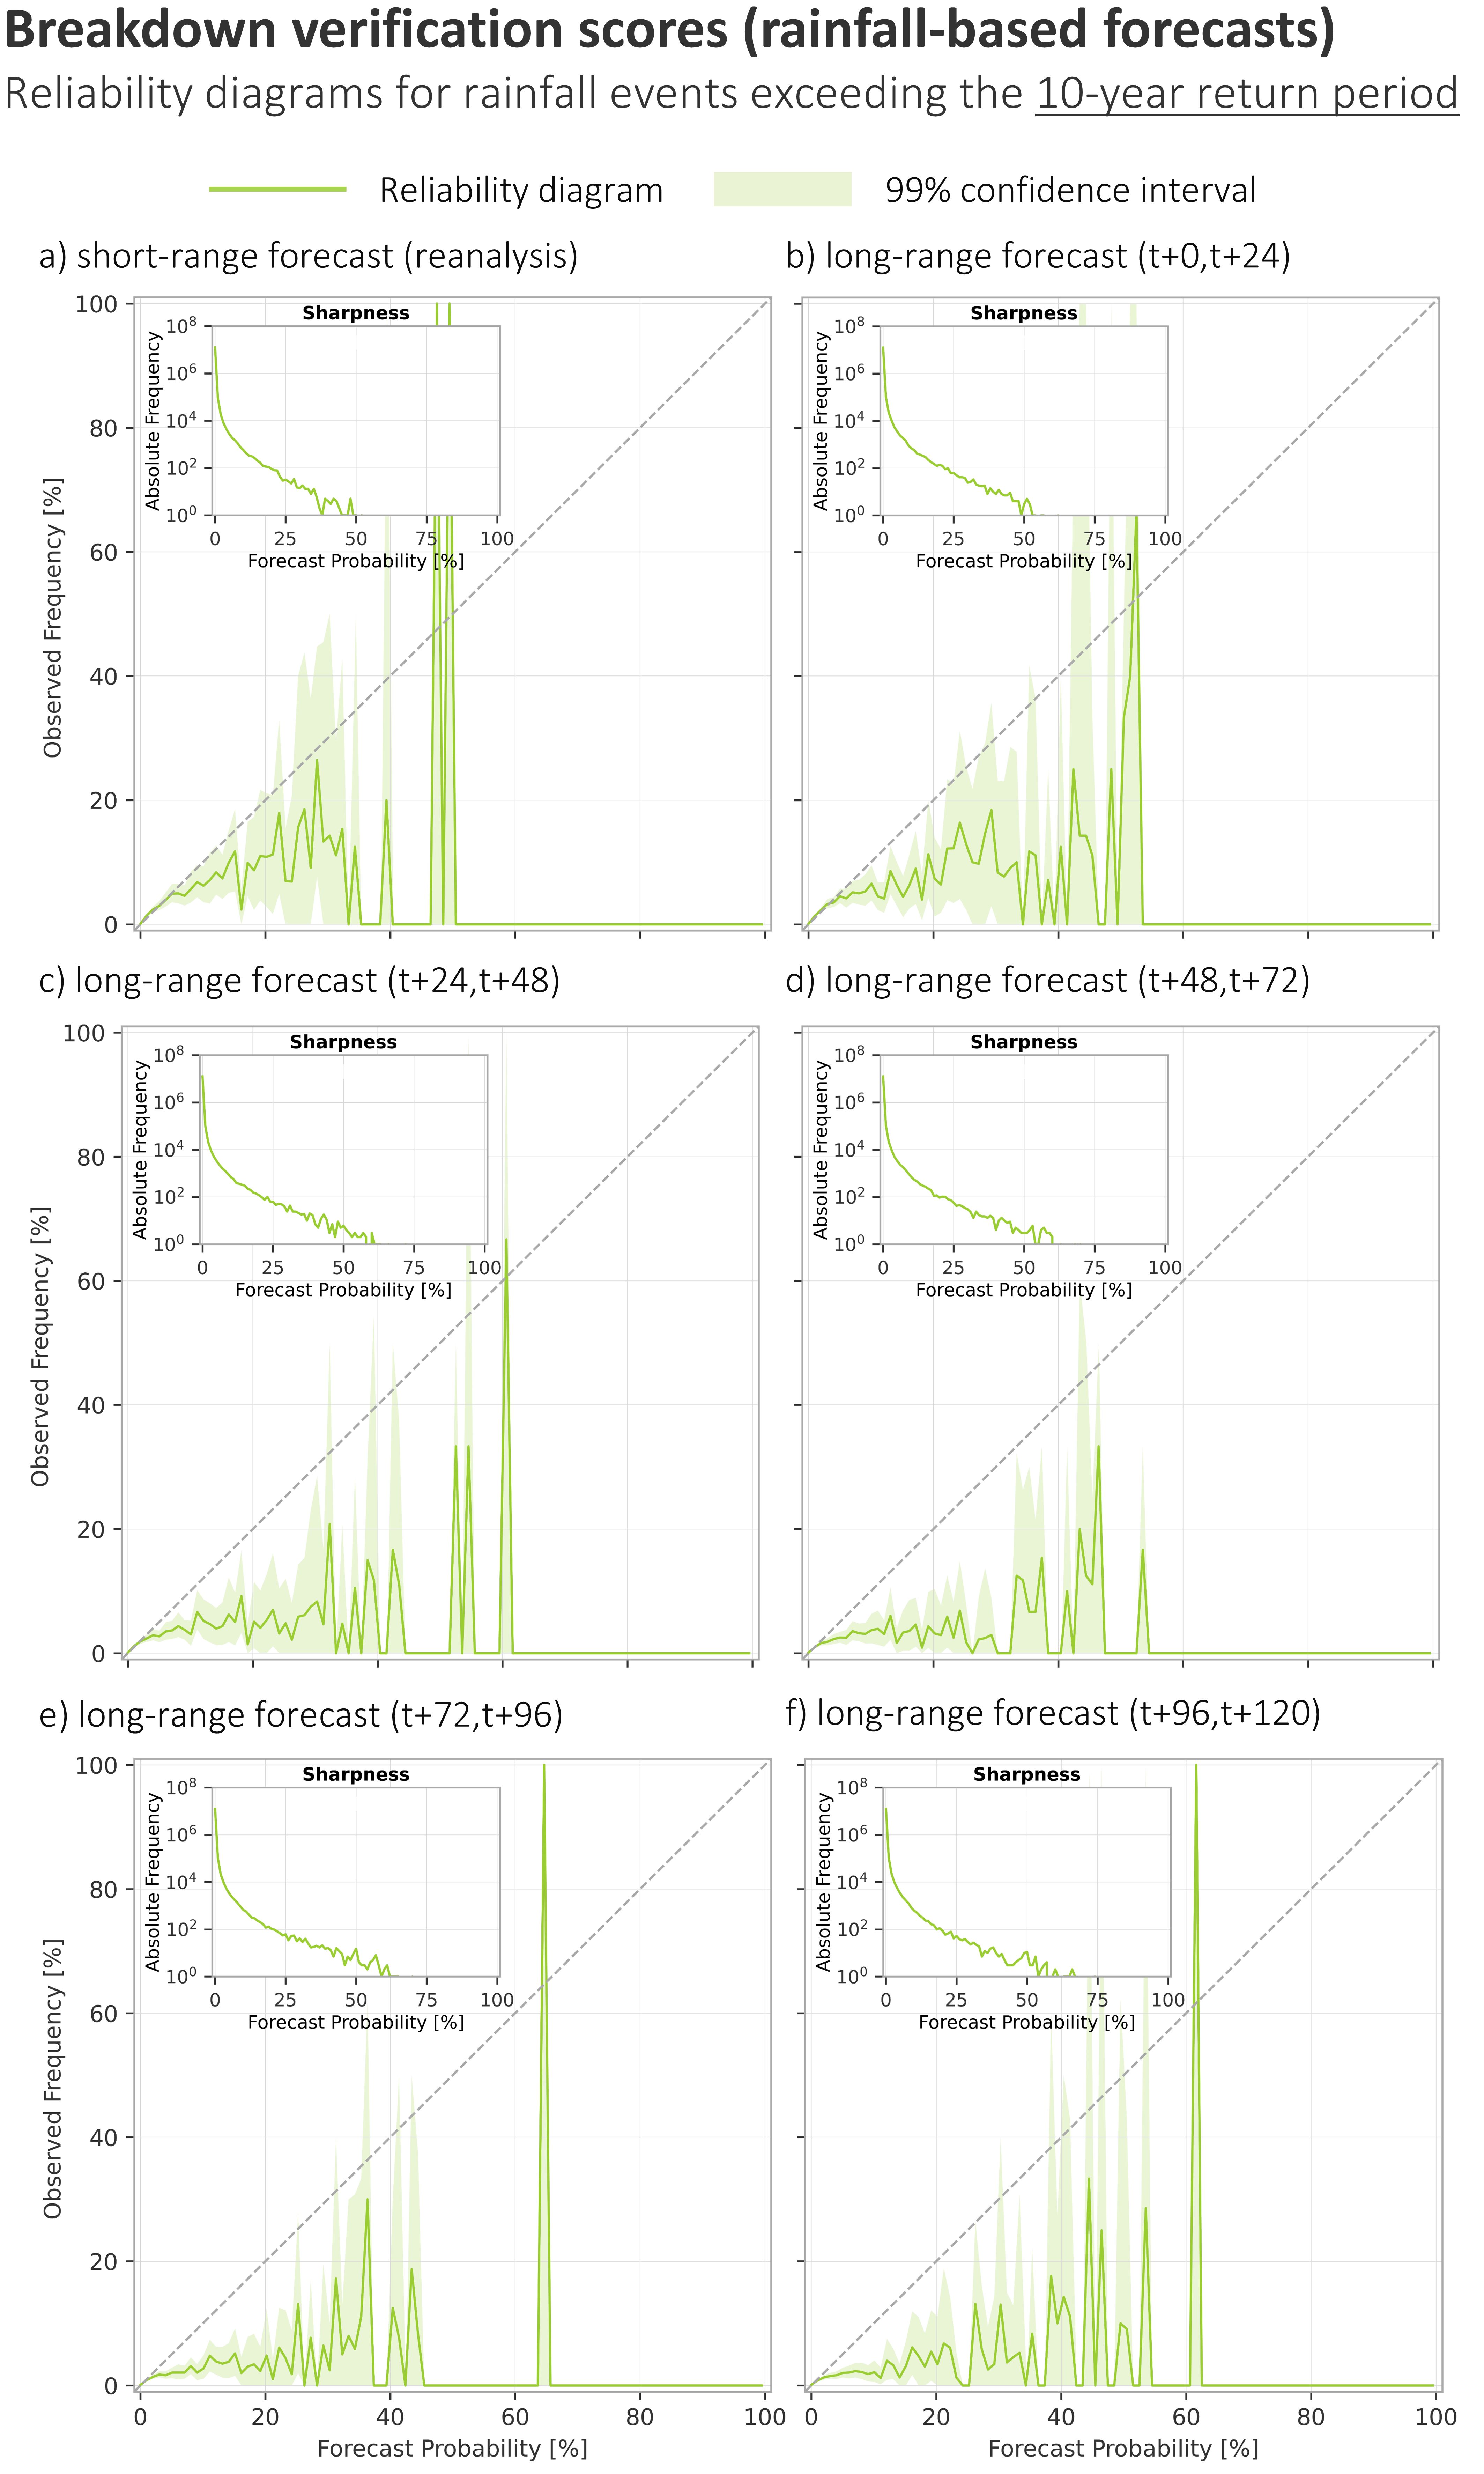
\includegraphics[width=\textwidth]{rainfall_based_ff_verif_breakdown_scores_rel_diag_10rp.png}
\caption{\textbf{Reliability diagrams for tp >= 5-year return period for the rainfall-based forecasts of areas at risk of flash floods built with ERA5-ecPoint.} Similar to Figure \ref{fig:rainfall_based_ff_verif_breakdown_scores_rel_diag_1rp}.}
\label{fig:rainfall_based_ff_verif_breakdown_scores_rel_diag_10rp}
\end{figure}

\begin{figure}[htbp]
\centering
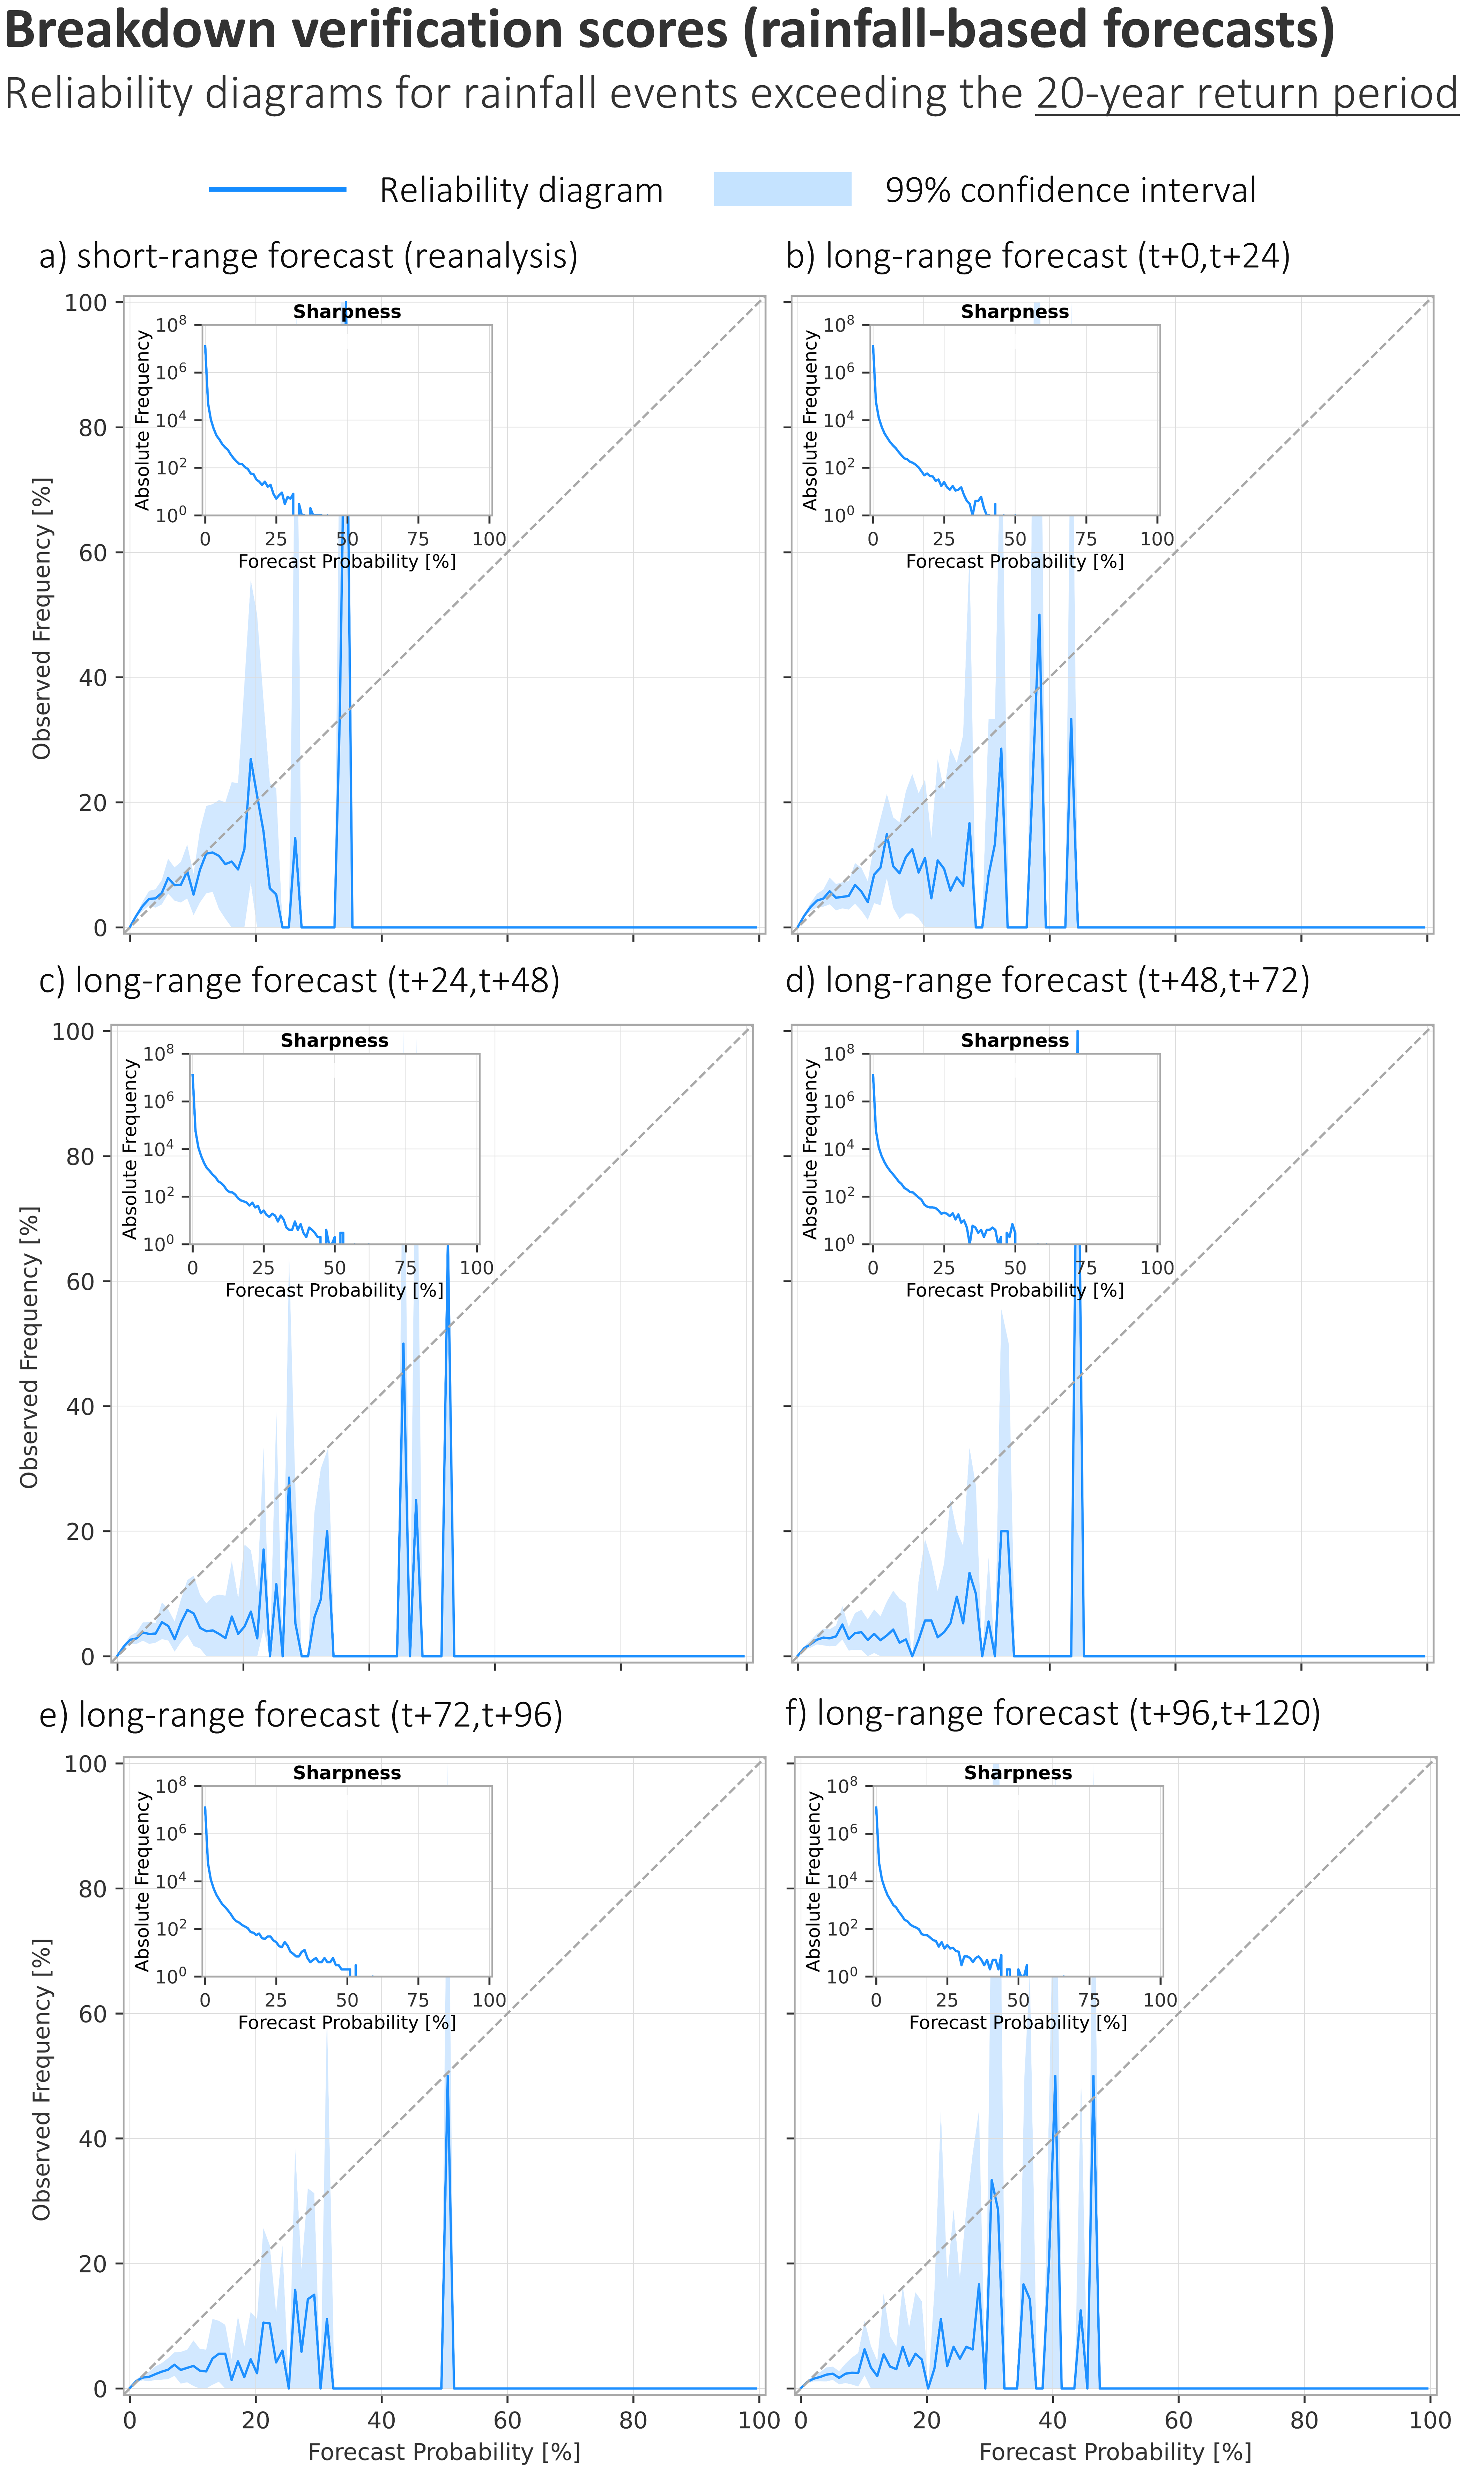
\includegraphics[width=\textwidth]{rainfall_based_ff_verif_breakdown_scores_rel_diag_20rp.png}
\caption{\textbf{Reliability diagrams for tp >= 5-year return period for the rainfall-based forecasts of areas at risk of flash floods built with ERA5-ecPoint.} Similar to Figure \ref{fig:rainfall_based_ff_verif_breakdown_scores_rel_diag_1rp}.}
\label{fig:rainfall_based_ff_verif_breakdown_scores_rel_diag_20rp}
\end{figure}

\begin{figure}[htbp]
\centering
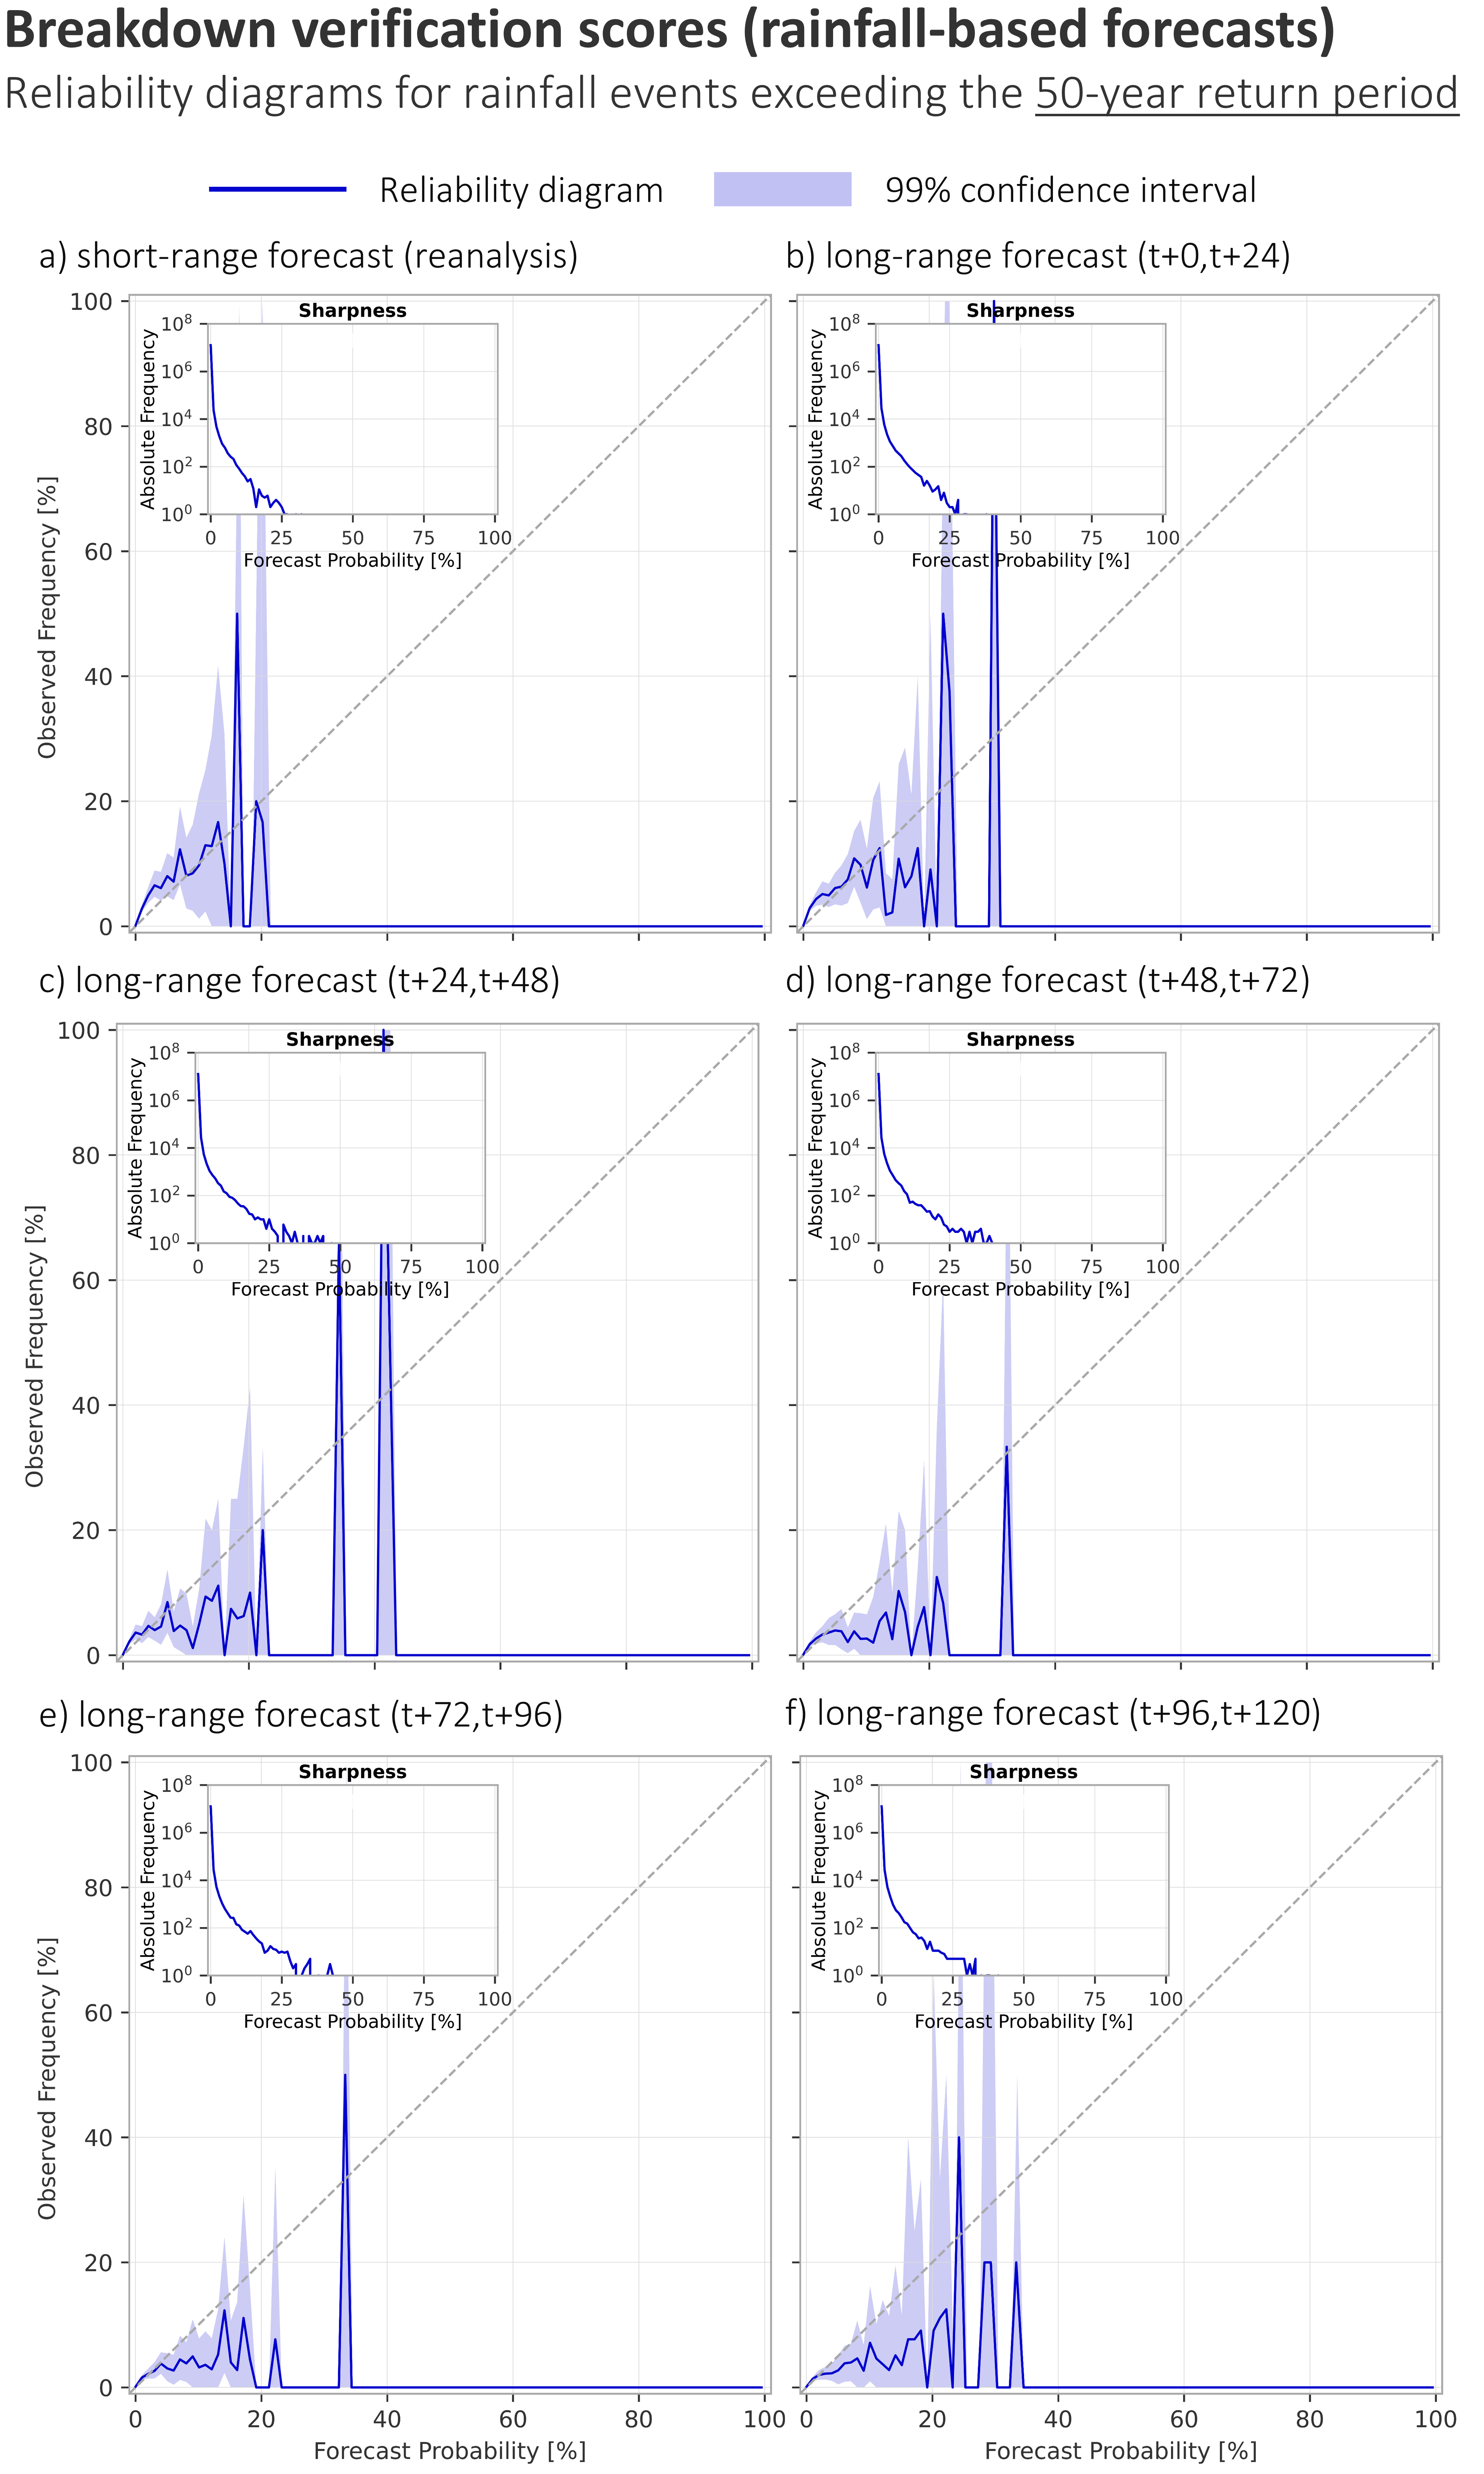
\includegraphics[width=\textwidth]{rainfall_based_ff_verif_breakdown_scores_rel_diag_50rp.png}
\caption{\textbf{Reliability diagrams for tp >= 5-year return period for the rainfall-based forecasts of areas at risk of flash floods built with ERA5-ecPoint.} Similar to Figure \ref{fig:rainfall_based_ff_verif_breakdown_scores_rel_diag_1rp}.}
\label{fig:rainfall_based_ff_verif_breakdown_scores_rel_diag_50rp}
\end{figure}

\begin{figure}[htbp]
\centering
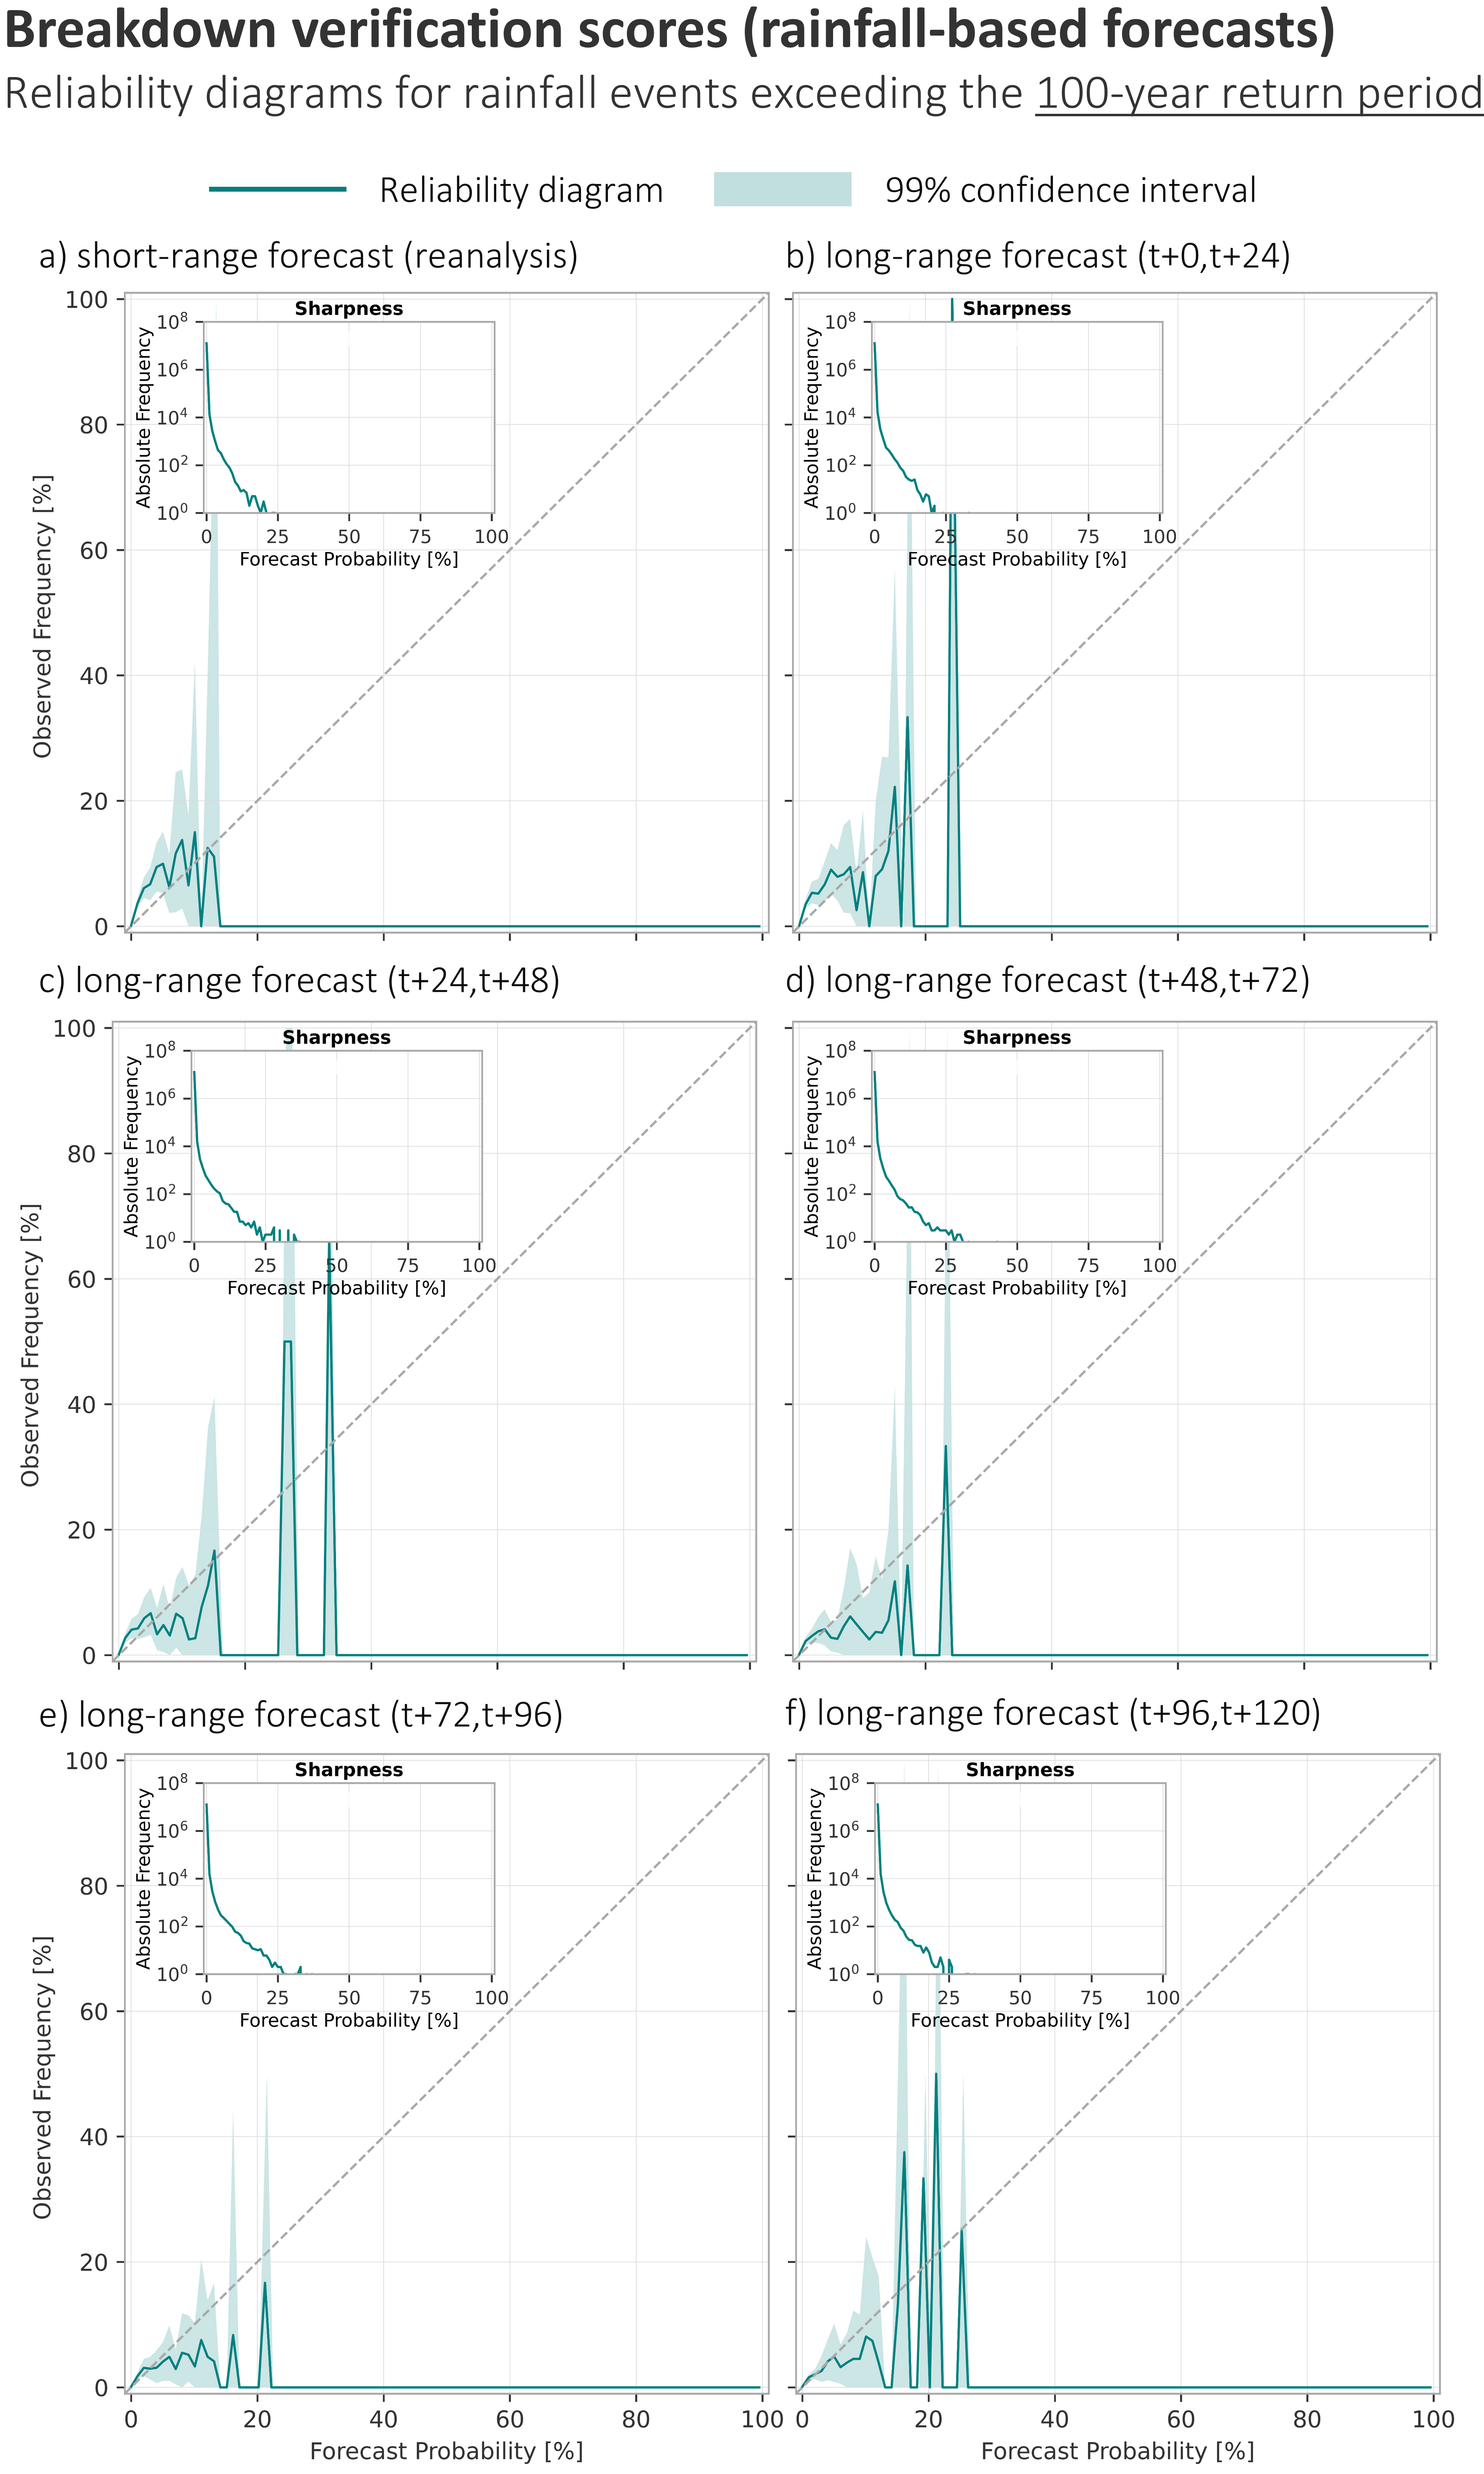
\includegraphics[width=\textwidth]{rainfall_based_ff_verif_breakdown_scores_rel_diag_100rp.png}
\caption{\textbf{Reliability diagrams for tp >= 5-year return period for the rainfall-based forecasts of areas at risk of flash floods built with ERA5-ecPoint.} Similar to Figure \ref{fig:rainfall_based_ff_verif_breakdown_scores_rel_diag_1rp}.}
\label{fig:rainfall_based_ff_verif_breakdown_scores_rel_diag_100rp}
\end{figure}


%%%%%%%%%%%%%%%%%%%%%
\section{Case Study: Storm Irma}
\label{flash_flood_focused_verification_rainfall_based_ff_CASE_STUDY}


%%%%%%%%%%%%%%%%%%%%%
\section{Discussions}
\label{flash_flood_focused_verification_rainfall_based_ff_DISCUSSIONS}


%%%%%%%%%%%%%%%%%%%%%
\section{Conclusions}
\label{flash_flood_focused_verification_rainfall_based_ff_CONCLUSIONS}
